\chapter{General Properties of Irrotational Motion in an Ideal Fluid (Potential Flows)}
\section{Basic Formulations of Potential Flows}
\subsection{Governing Equations}
Starting from irrotation: $\nabla\times\mathbf{v} = \mathbf{0}\Longrightarrow\mathbf{v} = \nabla\Phi$\\
For an ideal fluid, $\rho=$ constant, continuity equation: $\nabla\cdot\mathbf{v}=0$
\begin{equation}
\Longrightarrow\nabla\cdot\nabla\Phi = 0\Longrightarrow\boxed{\nabla^2\Phi = 0}\text{ (Laplace equation)}
\label{eq: 4-1-1}
\end{equation}
From Kelvin's circulation theorem
\[
\frac{D\Gamma}{Dt} =  0\text{ where }\Gamma = \oint_C\mathbf{v}\cdot\mathbf{t}dl
\]
hence if a flow field is circulation free flow (i.e. irrotational flow) initially, it will remain circulation free (i.e. irrotational) thereafter. The dynamics (i.e. pressure) of the flow field can be obtained from Bernoulli's equation, i.e.,
\begin{subequations}
\begin{align}
\frac{\partial\Phi}{\partial t} + \frac{p}{\rho} + \frac{1}{2}\nabla\Phi\cdot\nabla\Phi + U = f(t)
\label{eq: 4-1-2-a}
\end{align}
or redefine $\displaystyle\Phi \equiv\Phi-\int f(t)dt$
\begin{align}
\frac{\partial\Phi}{\partial t} + \frac{p}{\rho} + \frac{1}{2}\nabla\Phi\cdot\nabla\Phi + U = 0
\label{eq: 4-1-2-b}
\end{align}
\end{subequations}
Alternatively, staring from incompressibility: $\nabla\cdot\mathbf{v} = 0\Longrightarrow\mathbf{v} = \nabla\times\boldsymbol{\Psi}$\\
Use irrotaionality: $\nabla\times\mathbf{v} = \mathbf{0}$
\[
\Longrightarrow\nabla\times\left(\nabla\times\boldsymbol{\Psi}\right) = \mathbf{0}\Longrightarrow -\nabla^2\boldsymbol{\Psi} + \nabla\left(\nabla\cdot\boldsymbol{\Psi}\right) = \mathbf{0}
\]
\begin{note}
\[
\tilde{\boldsymbol{\Psi}} = \boldsymbol{\Psi} + \nabla A\Longrightarrow\nabla\times\tilde{\boldsymbol{\Psi}} = \nabla\times \boldsymbol{\Psi} + \cancelto{0}{\nabla\times\nabla A} = \mathbf{v}
\]
$\Longrightarrow\nabla\cdot\tilde{\boldsymbol{\Psi}} = \nabla\cdot\boldsymbol{\Psi} + \nabla^2A=0$, choose $A$ such that $\nabla^2A = -\nabla\cdot\boldsymbol{\Psi}$
\end{note}
Hence\footnote{Note that $\Psi$ is not uniquely determinated by $\mathbf{v}$}
\begin{equation}
\nabla^2\boldsymbol{\Psi} = 0
\label{eq: 4-1-3}
\end{equation}
\begin{enumerate}[label = (\alph*)]
\item For 2D flows\\
$\boldsymbol{\Psi} = \mathbf{e_z}\psi(x,y,t)$ only
\[
\Longrightarrow\nabla\cdot\boldsymbol{\Psi} = \frac{\partial\psi(x,y,t)}{\partial z} = 0
\]
therefore, governing equation: $\nabla\boldsymbol{\Psi} = 0\Longrightarrow\nabla^2\psi\mathbf{e_z} = \mathbf{0}$
\begin{equation}
\Longrightarrow\boxed{\nabla^2\psi = 0}
\end{equation}
(i.e. $\displaystyle\frac{\partial^2\psi}{\partial x^2} + \frac{\partial^2\psi}{\partial y^2} = 0$) (for 2D potential flow only))
\begin{exercise}{Show that for axisymmetric flows}\\
$\boldsymbol{\Psi}$ reduces to a vector of one component only and again $\nabla\cdot\boldsymbol{\Psi} = 0$, i.e.
\[
\boxed{\nabla^2\boldsymbol{\Psi} = 0}
\]
\begin{itemize}
\item for cylindrical coordinate ($r,z$)
\[
\nabla^2\left[\mathbf{e_\theta}\frac{1}{r}\psi(r,z,t)\right] = \mathbf{0}
\]
expanding:
\begin{equation}
\Longrightarrow\frac{\partial}{\partial r}\left(\frac{1}{r}\frac{\partial\psi}{\partial r}\right) + \frac{1}{r}\frac{\partial^2\psi}{\partial z^2} = 0
\label{eq: 4-1-4}
\end{equation}
(not a Laplace equation)
\item in spherical coordinate ($r,\theta$)
\[
\nabla^2\left[\mathbf{e_\varphi}\frac{1}{r\sin\theta}\psi(r,\theta,t)\right] = \mathbf{0}
\]
expanding:
\begin{equation}
\Longrightarrow\frac{\partial^2\psi}{\partial r^2} + \frac{\sin\theta}{r^2}\frac{\partial}{\partial\theta}\left(\frac{1}{\sin\theta}\frac{\partial\psi}{\partial\theta}\right) = 0
\label{eq: 4-1-4}
\end{equation}
\end{itemize}
\end{exercise}
\end{enumerate}
\subsection{Far-Field Boundary Conditions}
Consider the flow field generated by a solid body moving in an otherwise \emph{quiescent fluid}
\begin{tikzpicture}
    \filldraw[color=blue!60, fill=blue!10, tangent=0.1](0, 0) ellipse (1cm and 0.5cm);
    \draw[color=blue!60, pattern=hatch, pattern color=blue!60, hatch size=10pt, hatch angle=0](0,0) ellipse (1cm and 0.5cm);
    \draw [blue, ultra thick, use tangent, -latex] (0,0) -- (0,0.7) node [pos=0.7, anchor=east] {$\mathbf{n_S}$};
    \draw[color=blue!60, tangent=0.4](0, 0) ellipse (5cm and 4cm);
    \draw [blue, ultra thick, use tangent, -latex] (0,0) -- (0,-2) node [pos=1.0, anchor=east] {$\mathbf{n_{\Sigma}}$};
    \node[color=blue!60, above left] at ($(3,-3)$){$R$};
    \draw [color=blue!60, -{Latex[length=2mm]}, rotate=0] ($(4,0)$) arc [start angle=-190, end angle=-350, x radius=1.0cm, y radius=0.6cm] node [below] {$\Sigma$};
    \draw [color=blue!60, -{Latex[length=2mm]}, rotate=0] ($(0,0.2)$) arc [start angle=10, end angle=170, x radius=1.0cm, y radius=0.6cm] node [below] {$S$};
\end{tikzpicture}
\paragraph*{Neumann Extension Problem}\mbox{}\\
From divergence theorem
\[
\iiint_R\nabla^2\Phi d\volume = \oiint_S\mathbf{n_S}\cdot\nabla\Phi dS + \oiint_\Sigma\mathbf{n_{\Sigma}}\cdot\nabla\Phi d\Sigma
\]
\begin{align*}
\Longrightarrow
\oiint_\Sigma\mathbf{n_\Sigma}\cdot\nabla\Phi d\Sigma
&= -\oiint_S\underbrace{\mathbf{n_S}\cdot\nabla\Phi}_{=\mathbf{n}_S\cdot\mathbf{v_S\footnotemark}} dS \\
&= -\oiint_S\mathbf{n_S}\cdot\mathbf{v_S}dS = -\mathbf{v_S}\cdot\iint_S\mathbf{n_S}dS
\end{align*}
\footnotetext{no penetration on $S$}
i.e., 
\[
\oiint_\Sigma\mathbf{n_\Sigma}\cdot\nabla\Phi d\Sigma = 0
\]
Choose $\Sigma$ to be a large sphere with radius $r\to\infty$, then 
\[
\oiint_\Sigma\underbrace{\overbrace{\mathbf{n_Z}}^{=\mathbf{e}_r}\cdot\nabla\Phi}_{\displaystyle = \frac{\partial\Phi}{\partial r} = v_r}\overbrace{d\Sigma}^{=r^2\sin\theta d\theta d\varphi} = 0\Longrightarrow \oiint_\Sigma\underbrace{\frac{\partial\Phi}{\partial r}}_{=v_r}r^2\sin\theta d\theta d\varphi = 0
\]
\begin{equation}
\Longrightarrow v_r\equiv \frac{\partial\Phi}{\partial r}\sim o\left(\frac{1}{r^2}\right)
\end{equation}
Similarly, from divergence theorem\footnote{$\displaystyle\int_{\partial\mathcal{R}}\left(\cdot\right)n_idA = \int_\mathcal{R}\left(\cdot\right)_{,i}d\volume$}
\[
\iiint_R\cancelto{0}{\nabla\times\nabla\Phi}d\volume = \oiint_S\mathbf{n_S}\times\nabla\Phi dS + \oiint_\Sigma\mathbf{n_\Sigma}\times\nabla\Phi d\Sigma = 0
\]
\begin{align*}
\Longrightarrow
\oiint_\Sigma\mathbf{n_\Sigma}\times\nabla\Phi d\Sigma 
&= -\oiint_S\mathbf{n_S}\times\nabla\Phi dS = -\oiint_S\mathbf{n_S}\times\mathbf{v}dS\\ \
&\vc{=}{\cite{RN1}}{
\begin{subarray}{c}
  \text{p. 294-p. 296}\\
  \text{for circulation-free flow}
\end{subarray}
}0
\end{align*}
choose $\Sigma$ to be large sphere radius $r\to\infty$
\begin{multline*}
\oiint_\Sigma\mathbf{n_\Sigma}\times\nabla\Phi d\Sigma\\ = \oiint_\Sigma\mathbf{e_r}\times\left\{\cancelto{0}{\mathbf{e_r}\frac{\partial\Phi}{\partial r}} + \mathbf{e_\theta}\frac{1}{r}\frac{\partial\Phi}{\partial\theta} + \mathbf{e_\varphi}\frac{1}{r\sin\theta}\frac{\partial\Phi}{\partial\varphi}\right\}r^2\sin\theta d\theta d\varphi = 0
\end{multline*}
\begin{equation}
\Longrightarrow\underbrace{\frac{1}{r}\frac{\partial\Phi}{\partial\theta}}_{v_\theta},\underbrace{\frac{1}{r\sin\theta}\frac{\partial\Phi}{\partial \varphi}}_{v_\varphi}\sim o\left(\frac{1}{r^2}\right)\text{ as }r\to\infty
\end{equation}
\begin{exercise}{Show that for 2D flow (i.e. moving cylinder)}\mbox{}\\
B.C.'s at infinity:
\begin{align*}
v_r &\sim o\left(\frac{1}{r}\right) \\
v_\theta &\sim o\left(\frac{1}{r}\right)\text{ if }\Gamma = 0 \\
&\sim \mathcal{O}\left(\frac{1}{r}\right)\text{ if }\Gamma = 0
\end{align*}
\begin{proof}\mbox{}\\

\begin{tikzpicture}
    \filldraw[color=blue!60, fill=blue!10, tangent=0.6](0, 0) ellipse (1cm and 0.5cm);
    \draw[color=blue!60, pattern=hatch, pattern color=blue!60, hatch size=10pt, hatch angle=0](0,0) ellipse (1cm and 0.5cm);
    \coordinate (P) at ($(0, 0) + (20:1cm and 0.5cm)$);
    \coordinate (P') at ($(0, 0) + (30:1cm and 0.5cm)$);
    \coordinate (Q) at ($(0, 0) + (20:5cm and 4cm)$);
    \coordinate (Q') at ($(0, 0) + (30:5cm and 4cm)$);
    \draw[color=blue!60,-{Stealth[length=2mm]}, rotate=0] (0,0) [partial ellipse=30:150:5cm and 4cm];
    \draw[color=blue!60,-{Stealth[length=2mm]}, rotate=0] (0,0) [partial ellipse=150:270:5cm and 4cm];
    \draw[color=blue!60,-{Stealth[length=2mm]}, rotate=0] (0,0) [partial ellipse=270:380:5cm and 4cm];
    \draw[color=blue!60,->-=.5] (P') to  (Q');
    \draw[color=blue!60,->-=.5] (Q) to  (P);
    \draw[color=blue!60,-{Stealth[length=2mm]}, rotate=0] (0,0) [partial ellipse=20:-100:1cm and 0.5cm];
    \draw[color=blue!60,-{Stealth[length=2mm]}, rotate=0] (0,0) [partial ellipse=-100:-220:1cm and 0.5cm];
    \draw[color=blue!60,-{Stealth[length=2mm]}, rotate=0] (0,0) [partial ellipse=-220:-330:1cm and 0.5cm];
    \node[color=blue!60, above left] at ($(3,-3)$){$R$};
    \draw [color=blue!60, -{Latex[length=2mm]}, rotate=0] ($(0,0.2)$) arc [start angle=10, end angle=170, x radius=1.0cm, y radius=0.6cm] node [below] {$S$};
    \draw [blue, ultra thick, use tangent, -latex] (0,0) -- (1,0) node [right] {$\mathbf{t_S}$} ;
    \draw [blue, ultra thick, -latex] (5,0) -- (5,2) node [above] {$\mathbf{t_\Sigma}$} ;
    \draw [blue, ultra thick, -latex] (5,0) -- (6,3) node [above] {$\mathbf{v} = \nabla\Phi$} ;
    \node[blue, ultra thick , above left] at ($(5,0)$){$dl_\Sigma$};
\end{tikzpicture}\\
Consider circulation $\Gamma$ around solid cylinder, from Stokes' theorem
\begin{align*}
\oint_\Sigma\mathbf{t_\Sigma}\cdot\nabla\Phi dl_\Sigma
&= \iint_R\mathbf{n_z}\cdot\left(\nabla\times\nabla\Phi\right)dA_R - \oint_S\mathbf{t_S}\cdot\nabla\Phi dl_S = 0
\end{align*}
\[
\Longrightarrow
\oint_\Sigma\mathbf{t_\Sigma}\cdot\nabla\Phi dl_\Sigma = \oint_S\mathbf{t_S}\cdot\nabla\Phi dl_S\equiv \Gamma
\]
\begin{itemize}
\item if $\Gamma = 0$\\
\[
\oint_\Sigma\underbrace{\mathbf{t_\Sigma}}_{\mathbf{e_\theta}}\cdot\nabla\Phi dl_\Sigma = 0\Longrightarrow\oint_\Sigma\underbrace{\frac{1}{r}\frac{\partial\Phi}{\partial\theta}}_{v_\theta}rd\theta = 0
\]
\[
\Longrightarrow v_\theta \equiv \frac{1}{r}\frac{\partial\Phi}{\partial\theta}\sim o\left(\frac{1}{r}\right)\text{ as }r\to\infty
\]
\item if $\Gamma \neq 0$\\
\[
\Longrightarrow\oint_\Sigma\frac{1}{r}\frac{\partial\Phi}{\partial\theta}rd\theta = \Gamma
\]
\[
\Longrightarrow v_\theta \equiv \frac{1}{r}\frac{\partial\Phi}{\partial\theta}\sim \mathcal{O}\left(\frac{1}{r}\right)\text{ as }r\to\infty
\]
\end{itemize}
\begin{note}{For uniform stream past a fixed solid body}\mbox{}\\
\begin{tikzpicture} 
\draw[->] (-3,1) -- (-2,1) node [pos=0.5, anchor=south] {$\mathbf{v_\infty}$};
\draw[->] (-3,0) -- (-2,0);
\draw[->] (-3,-1) -- (-2,-1);
\filldraw[color=blue!60, fill=blue!10](0,0) circle (1);
\draw[color=blue!60, pattern=hatch, pattern color=blue!60, hatch size=10pt, hatch angle=0](0,0) circle (1);
\end{tikzpicture}\mbox{}\\
use coordinate transformation
\begin{align*}
\text{3D}&\colon \left(v_r-v_{\infty r}\right),\left(v_\theta-v_{\infty \theta}\right), \left(v_\varphi-v_{\infty \varphi}\right)\sim o\left(\frac{1}{r^2}\right)\text{ as }r\to\infty \\
\text{2D}&\colon \left(v_r-v_{\infty r}\right)\sim o\left(\frac{1}{r}\right), 
\end{align*}
\[
\begin{aligned}
\left(v_\theta-v_{\infty \theta}\right)
&\sim o\left(\frac{1}{r}\right) \text{ for }\Gamma=0\\
&\sim \mathcal{O}\left(\frac{1}{r}\right)\text{ for }\Gamma\neq 0
\end{aligned}
\text{ as }r\to\infty
\]
\end{note}
\end{proof}
\end{exercise}
\subsection{Physical Interpretation of the Velocity Potential Function $\Phi$}
Consider an irrotaional flow generated by a solid body which is set into motion \emph{impulsively from rest} ,i.e.
%----------------------
\begin{minipage}{0.4\textwidth}
\begin{align*}
\mathbf{v}=\mathbf{0} &\text{ at }t = 0\\
\mathbf{v}=\text{finite} &\text{ at }t = 0^+
\end{align*}
\end{minipage} \hfill
\begin{minipage}{0.5\textwidth}
\begin{tikzpicture}
\begin{axis}[xmin = -2, xmax= 2, ymin = -0.5, ymax= 1.2, axis lines = middle, xlabel = $t$, ylabel = $v$, title={},axis lines=center, axis line style={-{Latex[length=2mm]}}, scaled ticks=false,ytick={}, yticklabels={},xtick={}, xticklabels={}]
% \addplot[color=red, samples = 100]{exp(x)};
% \addplot [blue,thick] {func(x)};
\addplot[blue,thick, domain=-7:0] {0};
\addplot[blue,thick, domain=0:7] {1};
\end{axis}
\end{tikzpicture}
\end{minipage}\\
%----------------------
then
\[
\mathbf{v} = \lim_{t\to 0}\int_0^t\frac{\partial\mathbf{v}}{\partial t}dt
\]
From Bernoulli's equation
\[
\frac{\partial\mathbf{v}}{\partial t} + \nabla\underbrace{\left(\frac{v^2}{2}+\frac{p}{\rho} + U\right)}_{H} = 0
\]
hence
\[
\mathbf{v}=\lim_{t\to 0}-\int_0^t\nabla Hdt\Longrightarrow\nabla\Phi = \lim_{t\to 0}-\nabla\int_0^tHdt
\]
\[
\Longrightarrow\Phi = \lim_{t\to 0}-\int_0^tHdt
\]
\[
\text{for finite }\Phi\Longrightarrow H\to\infty\text{ at }t = 0^+\left[H = \cancelto{\text{finite at $t=0^+$}}{\frac{v^2}{2}}+\frac{p}{\rho} + \cancel{U}\right]
\]
Hence
\[
\Phi(\mathbf{x},t) = -\lim_{t\to 0}\int_0^t\frac{p}{\rho}dt\text{ with }p\to\infty\text{ as }t = 0^+
\]
(\emph{pressure impulse})
\section{Fundamental Solution and Green's Theorem}
\subsection{Fundamental Solution (of Laplace equation)}
\begin{itemize}
\item The Dirac Delta function $\delta(x)$ (unit impulse function)
\begin{definition}\mbox{}\\
$\delta(x) = 0$ for $x\neq 0$, $\delta(x)\to \infty$ at $x = 0$
\begin{equation}
\int_{-\infty}^\infty\delta(x) = 1
\label{eq: 4-2-1}
\end{equation}
\end{definition}
It's not an ordinary function, can approximate $\delta(x) $ as the limit of continuous function
\begin{enumerate}[label = \protect\circled{\arabic*}]
\item $\displaystyle d_n(x) = \frac{n}{\pi\left(1+n^2x^2\right)}$ as $n\to\infty$
\item $\displaystyle\frac{\epsilon}{\pi\left(x^2+\epsilon^2\right)}$ as $\epsilon\to\infty$
\item $\displaystyle\frac{1}{2\sqrt{\pi\epsilon}}e^{-\displaystyle\frac{x^2}{4\epsilon}}$ as $\epsilon\to 0$
\item $\displaystyle\frac{1}{2\left(\pi\right)^{3/2}\epsilon^3}e^{-\displaystyle\left(-\frac{r}{\epsilon}\right)^2}$ as $\epsilon\to 0$
\end{enumerate}
i.e. $\delta(r) = 0$ for $r\neq 0$, $\delta(r)\to\infty$ at $r=0$, and 
\[
{\oiint \hspace{-23.5pt} \int}_{\volume_\infty}\delta(r)d\volume = 1
\]
Operational definition of delta function
\begin{align*}
\int_{-\infty}^\infty\delta(x)f(x)dx = f(0), &&\text{or}&&\int_{-\infty}^\infty\delta(x-y)f(x)dx = f(y)
\end{align*}
$\delta(x)\colon$ sampling function, distribution, functional
\item Fundamental Solution (Green's function)\\
If a function $w$ satisfy a linear differential equation
\begin{equation}
Lu(x) = \delta(x-y)
\label{eq: 4-2-2}
\end{equation}
where $L$ denotes a linear differential operators of form,\\
e.g.
\[
a_n\frac{d^n}{dx^n} + a_{n-1}\frac{d^{n-1}}{dx^{n-1}} + \cdots + a_1\frac{d}{dx} + a_0
\]
or
\[
\frac{\partial^2}{\partial x^2} + \frac{\partial^2}{\partial y^2}
\]
e.g.
\begin{figure}[H]
\centering
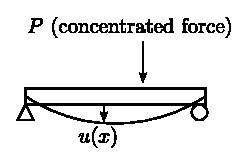
\includegraphics[scale=1.8]{figure/chapter4/4-1-1.eps}
%\caption{\label{fig:blue_rectangle} Rectangle}
\end{figure}
i.e. 
\[
Lw(x;y) = \delta(x-y)
\]
$w(x,y)$ is called the fundamental solution to the operator $L$\\
Consider an inhomogeneous linear differential equation
\begin{equation}
Lu(x) = f(x)
\label{eq: 4-2-3}
\end{equation}
The solution to \eqref{eq: 4-2-3} is
\begin{equation}
u(x) = \int_{-\infty}^\infty \underbrace{w(x;y)}_{
\begin{subarray}{c}
  \text{Kernal function}\\
  \text{transfer function}\\
  \text{influence function}
\end{subarray}
}f(y)dy
\label{eq: 4-2-3}
\end{equation}
\begin{proof}\mbox{}\\
from \eqref{eq: 4-2-3}
\begin{align*}
Lu(x)
&= L\int_{-\infty}^\infty w(x;y)f(y)dy \\
&= \int_{-\infty}^\infty \left[Lw(x;y)\right]f(y)dy \\
&= \int_{-\infty}^\infty \delta(x-y) f(y)dy =f(x)\\
\end{align*}
\[
\Longrightarrow Lw(x;y) = \delta(x-y)
\]
$w(x,y)$ is the \emph{response} of the system $L$ to an impulse input at $x=y$
\begin{figure}[H]
\centering
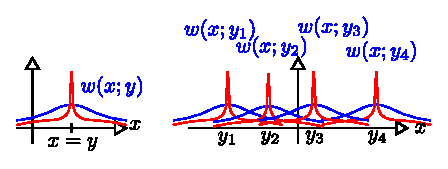
\includegraphics[scale=1.8]{figure/chapter4/4-1-2.eps}
%\caption{\label{fig:blue_rectangle} Rectangle}
\end{figure}
\end{proof}
\item Fundamental Solution to the Laplace equation\\
Consider
\begin{equation}
\nabla^2\phi = \delta(r)
\label{eq: 4-2-4}
\end{equation}
In spherical coordinate with spherical symmetry
\[
\nabla^2\equiv\frac{1}{r^2}\frac{\partial}{\partial r}\left(r^2\frac{\partial}{\partial r}\right)
\]
Guess $\displaystyle\phi = \frac{A}{r}$, $\nabla^2\phi = 0$ everywhere except at $r=0$ where $\phi$ is \emph{undefined} at $r=0$\\
Use integral definition of divergence
\[
\nabla^2\left(\frac{A}{r}\right)_{r=0}=\nabla\cdot\left(\nabla\frac{A}{r}\right)_{r=0} = \lim_{\Delta\volume\to 0}\frac{1}{\Delta\volume}\oiint_{\Delta S}\left(\nabla\frac{A}{r}\right)\cdot\mathbf{n}dS
\]
choose $\Delta\volume$ to be a sphere with radius $\epsilon\to 0$, then 
\[
\nabla\frac{A}{r} = -\frac{A}{r^2}\mathbf{e_r}
\]
and
\begin{align*}
\nabla^2\left(\frac{A}{r}\right)_{r=0}
&= \lim_{\Delta\volume\to 0}\frac{1}{\Delta\volume}\oiint_{\Delta S}-\frac{A}{r^2}\mathbf{e_r}\cdot\mathbf{n}dS \\
&= \lim_{\epsilon\to 0}\frac{-A}{\frac{4}{3}\pi\epsilon^3}\oiint_{\Delta S}\frac{1}{r^2}\underbrace{dS}_{=r^2\sin\theta d\theta d\varphi}\\
&= \lim_{\epsilon\to 0}\frac{-A}{\frac{4}{3}\pi\epsilon^3}\oiint_{\Delta \Omega}\frac{1}{r^2}\underbrace{r^2d\Omega}_{dS} \\
&= \lim_{\epsilon\to 0}\frac{-4\pi A}{\frac{4}{3}\pi\epsilon^3} \to \infty
\end{align*}
i.e., $\displaystyle\nabla^2\left(\frac{A}{r}\right)$ behaves like $\delta(r)$.\\
What is $A$?\\
Recall 
\[
{\oiint \hspace{-23.5pt} \int}_{\volume(\infty)}\delta(r)d\volume\equiv 1, {\oiint \hspace{-23.5pt} \int}_{\volume(\epsilon)}\delta(r)d\volume= 1
\]
but 
\[
{\oiint \hspace{-23.5pt} \int}_{\volume(\infty)}\nabla^2\left(\frac{A}{r}\right)d\volume\equiv{\oiint \hspace{-23.5pt} \int}_{\volume(\epsilon)}\nabla^2\left(\frac{A}{r}\right)d\volume = \nabla^2\left(\frac{A}{r}\right)_{r=0}\underbrace{\volume(\epsilon)}_{\frac{4}{3}\pi\epsilon^3} = 1
\]
\[
\Longrightarrow A = -\frac{1}{4\pi}
\]
i.e. solution to \eqref{eq: 4-2-4} is 
\begin{equation}
\boxed{\phi = -\frac{1}{4\pi r}}\text{ (fundamental solution)}
\label{eq: 4-2-5}
\end{equation}
\begin{exercise}{Show that 2D fundamental solution to the Laplace equation is}
\[
\boxed{\phi = \frac{1}{2\pi}\ln r}
\]
\end{exercise}
\end{itemize}
\subsection{Green's Theorem (Green's Identities) (Green's Formula)}
\begin{itemize}
\item Green's 2\textsuperscript{nd} identity
\begin{equation}
{\oiint \hspace{-23.5pt} \int}_{\volume}\left(\phi'\nabla^2\phi-\phi\nabla^2\phi'\right)d\volume = \oiint_S\left(\phi'\frac{\partial\phi}{\partial n} - \phi\frac{\partial\phi'}{\partial n}\right)dS
\label{eq: 4-2-6}
\end{equation}
both $\phi$ and $\phi'$ are continuous and differentiable scalar function.
\item Application of Green's Theorem\\
Use Green's theorem to express $\phi$ in $\volume$, which satisfies $\nabla^2\phi = 0$, in terms of boundary data on $S$. (This is equivalent to solve $\nabla^2\phi = 0$ in $\volume$ with B.C.'s, $\displaystyle\frac{\partial \phi}{\partial n},\phi$ on $S$.)\\
Let $\phi' = 1/r$, the $\nabla^2\phi' = 0$ everywhere except at $r=0$.\\
Hence
\[
{\oiint \hspace{-23.5pt} \int}_{\volume}\phi'\nabla^2\phi d\volume \vc{=}{\text{if}}{\nabla^2\phi =0} 0, 
\]
\[
{\oiint \hspace{-23.5pt} \int}_{\volume}\phi\nabla^2\phi'\equiv{\oiint \hspace{-23.5pt} \int}_{\volume}\phi\nabla^2\left(\frac{1}{r}\right)d\volume \neq 0\text{ if the point $r=0$ is inside $\volume$}
\]
Recall that
\[
{\oiint \hspace{-23.5pt} \int}_{\volume}\underbrace{\nabla^2\left(-\frac{1}{4\pi r}\right)}_{\sim\delta (r)}d\volume\equiv 1
\]
\[
\therefore{\oiint \hspace{-23.5pt} \int}_{\volume}\phi\nabla^2\left(\frac{1}{r}\right)d\volume = -4\pi{\oiint \hspace{-23.5pt} \int}_{\volume}\phi\underbrace{\nabla^2\left(-\frac{1}{4\pi r}\right)}_{\sim\delta(r)}d\volume = -4\pi\phi_0
\]
where $\phi_0$ is the value of $\phi$ at $r = 0$\\
and
\begin{equation}
\eqref{eq: 4-2-6}\Longrightarrow\oiint_S\left[\frac{1}{r}\frac{\partial\phi}{\partial n} - \phi\frac{\partial}{\partial n}\left(\frac{1}{r}\right)\right]dS
\text{(Green's formula)}
\label{eq: 4-2-7}
\end{equation}
Given $\frac{\partial\phi}{\partial n}, \phi$ on $S$, \eqref{eq: 4-2-7} gives $\phi_0$ at any point in $\volume$.\\
In practice, the use of \eqref{eq: 4-2-7} is 
\begin{tikzpicture}
    % Axes
    \draw [arrows = {-Latex[color=black, fill=white, length=3mm]}] (0,0,0) -- (2,0,0) node [at end, right] {$x$};
    \draw [arrows = {-Latex[color=black, fill=white, length=3mm]}] (0,0,0) -- (0,2,0) node [at end, left] {$y$};
    \draw [arrows = {-Latex[color=black, fill=white, length=3mm]}] (0,0,0) -- (0,0,2) node [at end, left] {$z$};
    \draw[-](3, 3) ellipse (3cm and 2cm);
    \draw [-{Latex[length=2mm]}, rotate=0] (0,0) -- (3,4) node[above]{$P$} node[pos=0.7, anchor=east] {$\mathbf{r_p}$};
    \draw [-{Latex[length=2mm]}, rotate=0] (0,0) -- (2,4.5) node[pos=0.7, anchor=east] {$\mathbf{r'}$};
\end{tikzpicture}
\begin{equation}
4\pi\phi_P = \oiint_S\left[\frac{1}{r}\frac{\partial\phi}{\partial n} - \phi\frac{\partial}{\partial n}\left(\frac{1}{r}\right)\right]dS
\label{eq: 4-2-8}
\end{equation}
where $\displaystyle r = \frac{1}{\abs{\mathbf{r'}-\mathbf{r_p}}}$
\begin{exercise}{For 2D case}
\begin{equation}
-2\pi\phi_P = \oint_C\left[\ln\frac{\partial\phi}{\partial n} - \phi\frac{\partial}{\partial n}\left(\ln r\right)\right]dl
\label{eq: 4-2-9}
\end{equation}
\end{exercise}
\end{itemize}
\newpage
\paragraph*{Modification for the problem involving a solid-body moving in infinite domain (Neumann Exterior Boundary)}
\begin{tikzpicture}
    \filldraw[color=blue!60, fill=blue!10, tangent=0.1](0, 0) ellipse (1cm and 0.5cm);
    \draw[color=blue!60, pattern=hatch, pattern color=blue!60, hatch size=10pt, hatch angle=0](0,0) ellipse (1cm and 0.5cm);
    \draw [blue, ultra thick, use tangent, -latex] (0,0) -- (0,0.7) node [pos=0.7, anchor=east] {$\mathbf{n_S}$};
    \node[blue, ultra thick, below left ] at ($(0,0)$){$\mathbf{\volume_S}$};
    \draw[color=blue!60, tangent=0.4](0, 0) ellipse (5cm and 4cm);
    \draw [blue, ultra thick, use tangent, -latex] (0,0) -- (0,-2) node [pos=1.0, anchor=east] {$\mathbf{n_{\Sigma}}$};
    \filldraw [color=red, fill=red] (3,-1) circle (0.1) node [below right] at  ($(3,-1)$){$P$} ;
    \coordinate (P') at ($(0,0)+(-110:5 and 4)$) ;
    \draw[color=red, -{Latex[length=2mm]}, rotate=0] ($(3,-1)$) -- (P') node [pos=0.5, anchor=south] {$\mathbf{R}$};
    \coordinate (P'') at ($(0,0)+(-70:1 and 0.5)$) ;
    \draw[color=red, -{Latex[length=2mm]}, rotate=0] ($(3,-1)$) -- (P'') node [pos=0.5, anchor=south] {$\mathbf{r}$};
    \draw[transparent, tangent=0.1](0, 0) ellipse (1cm and 0.5cm);
    \draw [blue, ultra thick, use tangent, -latex] (0,0) -- (0,-0.7) node [pos=1.0, anchor=east] {$\mathbf{n = -n_S}$};
    \filldraw [color= yellow!80!black, fill=yellow!80!black, rotate around={-60:(3,1)}] (3,1) rectangle (2,0.5) node [color = yellow!70!black, pos=1.0, anchor=east] {$d\Sigma$};
    \draw[color=yellow!70!black, ultra thick, -{Latex[length=2mm]}, rotate around={-60:(3,1)}] (2.5,0.7) -- (2.5,2) node [pos = 1.0, anchor=south] {$\mathbf{n_\Sigma}$};
    \draw [color=blue!60, -{Latex[length=2mm]}, rotate=0] ($(4,0)$) arc [start angle=-190, end angle=-350, x radius=1.0cm, y radius=0.6cm] node [below] {$\Sigma$};
    \draw [color=blue!60, -{Latex[length=2mm]}, rotate=0] ($(0,0.2)$) arc [start angle=10, end angle=170, x radius=1.0cm, y radius=0.6cm] node [below] {$S$};
\end{tikzpicture}

Consider $\nabla^2\phi = 0$ and $\phi\to\phi_\infty$ as $R\to\infty$ or $\displaystyle\nabla\phi\to 0\left(\nabla\phi\sim o\left(\frac{1}{R^2}\right)\right)$\\
\eqref{eq: 4-2-8} is modified to 
\begin{equation}
\begin{aligned}
4\pi\phi_P
&= \oiint_S\left[\frac{1}{r}\frac{\partial\phi}{\partial n_S} - \phi\frac{\partial}{\partial n_S}\left(\frac{1}{r}\right)\right]dS \\
&+ \oiint_\Sigma\left[\frac{1}{R}\frac{\partial\phi}{\partial n_\Sigma} - \phi\frac{\partial}{\partial n_\Sigma}\left(\frac{1}{R}\right)\right]
\end{aligned}
\tag{$\ast$}
\label{eq: 4-2-9-*}
\end{equation}
Choose $\Sigma$ to be a large sphere with radius $R\to\infty$
\[
\oiint_\Sigma\frac{1}{R}\frac{\partial\phi}{\partial n_\Sigma}d\Sigma = \iint\frac{1}{R}\frac{\partial\phi}{\partial R}\underbrace{R^2\sin\theta d\theta d\varphi}_{d\Sigma}\to 0\text{ as }R\to \infty
\]
\begin{align*}
\oiint_\Sigma\phi\frac{\partial}{\partial n_\Sigma}\left(\frac{1}{R}\right)d\Sigma
&= \oiint_\Sigma\phi\frac{\partial}{\partial R}\left(\frac{1}{R}\right)d\Sigma \\
&= - \oiint_\Sigma \frac{\phi}{R^2} \underbrace{d\Sigma}_{=R^2d\Omega} = -\oiint_\Omega \phi d\Omega = -4\pi \phi_\infty
\end{align*}
Hence
\begin{equation}
\begin{aligned}
\eqref{eq: 4-2-9-*} \Longrightarrow
4\pi\left(\phi_P-\phi_\infty\right)
&= \oiint_S\left[\frac{1}{r}\frac{\partial\phi}{\partial n_S} - \phi\frac{\partial}{\partial n_S}\left(\frac{1}{r}\right)\right]dS \\
&= \oiint_S\left[-\frac{1}{r}\frac{\partial\phi}{\partial n} + \phi\frac{\partial}{\partial n}\left(\frac{1}{r}\right)\right]dS
\end{aligned}
\label{eq: 4-2-10}
\end{equation}
\begin{exercise}{For 2D case}
\begin{equation}
-2\pi\left(\phi_P-\phi_\infty\right) = \oint_C\left[-\ln r\frac{\partial\phi}{\partial n} + \phi\frac{\partial}{\partial n}\left(\ln r\right)\right]dl
\end{equation}
\end{exercise}
\begin{itemize}
\item Interpretation of \eqref{eq: 4-2-10}\\
Let us identity $\phi$ with the velocity potential function $\Phi$
\[
\nabla^2\Phi = 0
\]
Imagine the solid body is replaced by another potential flow with velocity potential $\hat{\Phi}$
\[
\boxed{\nabla^2\hat{\Phi} = 0}
\]
\begin{equation}
\begin{aligned}
&\oiint_S\left[\frac{1}{r}\frac{\partial\hat{\Phi}}{\partial n} - \hat{\Phi}\frac{\partial}{\partial n}\left(\frac{1}{r}\right)\right]dS \\ 
= &{\oiint \hspace{-23.5pt} \int}_{\volume_S}\left[\frac{1}{r}\cancelto{0}{\nabla^2\hat{\Phi}}-\hat{\Phi}\cancelto{0}{\nabla^2\left(\frac{1}{r}\right)}\right]d\volume
\end{aligned}
\label{eq: 4-2-11}
\end{equation}
From \eqref{eq: 4-2-10} + \eqref{eq: 4-2-11}
\begin{equation}
\begin{aligned}
\Longrightarrow
&4\pi\left(\Phi_P-\Phi_\infty\right) \\ = &\oiint_S\left[\left(\Phi - \hat{\Phi}\right)\frac{\partial}{\partial n}\left(\frac{1}{r}\right) + \frac{1}{r}\left(\frac{\partial\hat{\Phi}}{\partial n} - \frac{\partial\Phi}{\partial n}\right)\right]dS
\end{aligned}
\label{eq: 4-2-12}
\end{equation}
Since $\hat{\Phi}$ can be any potential flow, in 2 choice
\begin{enumerate}[label = (\alph*)]
\item If $\hat{\Phi} = \Phi$ on $S$ (but $\displaystyle\frac{\partial \hat{\Phi}}{\partial n}\neq\frac{\partial\Phi}{\partial n}$ on $S$)\\
$\eqref{eq: 4-2-11}\Longrightarrow$
\begin{equation}
\begin{aligned}
4\pi\left(\Phi_P-\Phi_\infty\right) &= \oiint_S\frac{\displaystyle\left(\frac{\partial\hat{\Phi}}{\partial n} - \frac{\partial\Phi}{\partial n}\right)}{r}dS\\ &= \oiint_S\frac{A(S)}{r}dS
\end{aligned}
\label{eq: 4-2-13}
\end{equation}
$A(S)dS\equiv$ strength of the distributed source/sink over $dS$\\
e.g. Panel method
\begin{figure}[H]
\centering
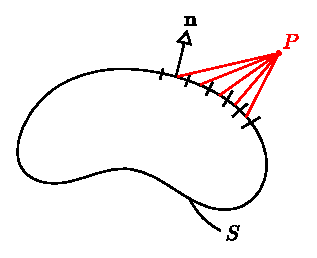
\includegraphics[scale=1.8]{figure/chapter4/4-1-3.eps}
%\caption{\label{fig:blue_rectangle} Rectangle}
\end{figure}
\item If $\displaystyle\frac{\partial \hat{\Phi}}{\partial n}=\frac{\partial\Phi}{\partial n}$ on $S$\\
$\eqref{eq: 4-2-11}\Longrightarrow$
\begin{equation}
\begin{aligned}
4\pi\left(\Phi_P-\Phi_\infty\right) &= \oiint_S\left(\Phi-\hat{\Phi}\right)\frac{\partial}{\partial n}\left(\frac{1}{r}\right)dS \\
&= \oiint_SB(S)\frac{\partial}{\partial n}\left(\frac{1}{r}\right)dS
\end{aligned}
\label{eq: 4-2-14}
\end{equation}
\end{enumerate}
\end{itemize}
\subsection{Irrotational Motion and Circulation}
Irrotational (i.e. $\nabla\times\mathbf{v}=\mathbf{0}\xcancel{\Longrightarrow}\Gamma_C(\equiv\oint_C\mathbf{v}\cdot\mathbf{t}dl)\footnotemark =0$ in $R$ everywhere)\footnotetext{around any circuit $C$ in $R$}\\
\begin{center}
\begin{tikzpicture} 
    \filldraw[color=blue!60, fill=blue!10](0,0) ellipse (1cm and 0.5cm);
    \draw[color=blue!60, pattern=hatch, pattern color=blue!60, hatch size=10pt, hatch angle=0](0,0) circle (1cm and 0.5cm);
    \draw [-{Latex[length=2mm]}, rotate=0] (1.5,0) arc [start angle=-20, end angle=350, x radius=1.5cm, y radius=1.2cm] node [above right] {$C$} node [below right] {$\Gamma_C\neq 0$};
    \draw [-{Latex[length=2mm]}, rotate=0] (3,-2) arc [start angle=-20, end angle=350, x radius=0.7cm, y radius=0.5cm] node [below right] {$\Gamma_C = 0$};
\end{tikzpicture}
\end{center}
\subsubsection{Some Topological Notions}
\begin{itemize}
\item Connectivity\\
A region $R$ is said to be \emph{connected} if any two points in $R$ can be connected by a continuous curve that does not leave $R$.\\
%----------------------
\begin{minipage}{0.4\textwidth}
\begin{tikzpicture} 
    \draw[thick](0,0) circle (1cm and 0.5cm) node [right] {$R$};
    \node at (1.5,0) {$R'$};
    \draw  ($(0,0)+(-70:1 and 0.5)$) .. controls +(down:2mm) and +(left:1mm) .. (1,-0.8) node[right]{$S$} ;
\end{tikzpicture}
\end{minipage} \hfill
\begin{minipage}{0.4\textwidth}
\begin{align*}
R&\colon\text{ connected}\\
R'&\colon\text{ connected}\\
R\cup R'\setminus S&\colon\text{ not a connected region}\\
\end{align*}
\end{minipage}\\
%----------------------
\item Reducible and irreducible circuits\\
If a circuit can be continuously contracted to a point without ever leaving $R$, the circuit is said to be reducible, otherwise, irreducible.\\
In 3D\\
%----------------------
\begin{minipage}{0.4\textwidth}
\begin{tikzpicture} 
    \filldraw[color=blue!60, fill=blue!10](0,0) ellipse (1cm and 0.5cm);
    \draw[color=blue!60, pattern=hatch, pattern color=blue!60, hatch size=10pt, hatch angle=0](0,0) circle (1cm and 0.5cm);
    \draw [thick,-, rotate=0] (1.5,0) arc [start angle=-20, end angle=350, x radius=1.5cm, y radius=1.2cm] node [above right] {$C_2$};
    \draw [thick,-, rotate=0] (4,0) arc [start angle=-20, end angle=350, x radius=0.7cm, y radius=0.5cm] node [below right] {$C_1$};
\end{tikzpicture}
\end{minipage} \hfill
\begin{minipage}{0.4\textwidth}
\begin{align*}
C_1&\colon\text{ reducible}\\
C_2&\colon\text{ reducible}
\end{align*}
\end{minipage}\\
%----------------------
In 2D\\
%----------------------
\begin{minipage}{0.4\textwidth}
\begin{tikzpicture} 
    \filldraw[color=blue!60, fill=blue!10](0,0) ellipse (1cm and 0.5cm);
	\draw[color=blue!60, pattern={Lines[angle=45,distance=5pt]}, pattern color=blue!60](0,0) circle (1cm and 0.5cm);
    \draw [thick,-, rotate=0] (1.5,0) arc [start angle=-20, end angle=350, x radius=1.5cm, y radius=1.2cm] node [above right] {$C_2$};
    \draw [thick,-, rotate=0] (4,0) arc [start angle=-20, end angle=350, x radius=0.7cm, y radius=0.5cm] node [below right] {$C_1$};
\end{tikzpicture}
\end{minipage} \hfill
\begin{minipage}{0.4\textwidth}
\begin{align*}
C_1&\colon\text{ reducible}\\
C_2&\colon\text{ irreducible}
\end{align*}
\end{minipage}\\
%----------------------
In 3D (torus)\\
%----------------------
\begin{minipage}{0.4\textwidth}
\begin{tikzpicture}
\begin{scope}[rotate=0]
%draw right C3
    \draw[thick,-, rotate=0] (1.5,0) [partial ellipse=60:185:0.6cm and 1.4cm];
    \draw[thick,dashed,-, rotate=0] (1.5,0) [partial ellipse=185:250:0.6cm and 1.4cm];
    \draw[thick,-, rotate=0] (1.5,0) [partial ellipse=250:300:0.6cm and 1.4cm] node [below right] {$C_3$};
    \draw[thick,dashed,-, rotate=0] (1.5,0) [partial ellipse=300:420:0.6cm and 1.4cm];
    \draw[thick,-, rotate=0] (-1.9,0) [partial ellipse=60:300:0.6cm and 1.4cm] node [below]{$C_2$};
    \draw[thick,dashed,-, rotate=0] (-1.9,0) [partial ellipse=300:420:0.6cm and 1.4cm];
    \draw [thick,-, rotate=0] (5,0) arc [start angle=-20, end angle=350, x radius=0.7cm, y radius=0.5cm] node [below right] {$C_1$};
    % \draw[thick,-, rotate=0] (-1.9,0) [partial ellipse=360:365:0.6cm and 1.4cm];
    \draw (0,0) ellipse (3 and 1.5);
    \clip (0,-1.8) ellipse (3 and 2.5);
    \draw (0,2.2) ellipse (3 and 2.5);
    \clip (0,2.2) ellipse (3 and 2.5);
    \draw (0,-2.2) ellipse (3 and 2.5);
\end{scope}
\end{tikzpicture}
\end{minipage} \hfill
\begin{minipage}{0.4\textwidth}
\begin{align*}
C_1&\colon\text{ reducible}\\
C_2&\colon\text{ reducible}\\
C_3&\colon\text{ irreducible}
\end{align*}
\end{minipage}\\
%----------------------
\item Simply-Connected Region (SCR)\\
A connected region in which all circuit are reducible.
\item Doubly-Connected Region (DCR)\\
%----------------------
\begin{minipage}{0.2\textwidth}
\begin{tikzpicture} 
    \filldraw[color=blue!60, fill=blue!10](0,0) ellipse (1cm and 0.5cm);
    \draw[color=blue!60, pattern={Lines[angle=45,distance=5pt]}, pattern color=blue!60](0,0) circle (1cm and 0.5cm);
    \node [below right] at (0.5,-0.5){$R$};    
\end{tikzpicture}
\end{minipage} \hfill
\begin{minipage}{0.45\textwidth}
\begin{tikzpicture} 
\begin{scope}[rotate=30]
\node[cylinder, 
    draw = violet, 
    text = purple,
    cylinder uses custom fill, 
    cylinder body fill = magenta!10, 
    cylinder end fill = magenta!40,
    aspect=1.5, rotate=30,
    minimum height=5cm, minimum width=1cm] (c) at (0,0) {};
    \draw[thick,-, rotate=0] (1.5,0) [partial ellipse=25:335:0.6cm and 1.3cm];
\draw[thick,dashed,-, rotate=0] (1.5,0) [partial ellipse=335:385:0.6cm and 1.3cm] ;
\draw[thick, ->] (-2,0)--(-4,0) node[above left] {$-\infty$};
\draw[thick, ->] (2.5,0)--(4.5,0) node[above] {$-\infty$};
\end{scope}
\coordinate (C) at ($(1.5,0)+(250:0.6 and 1.3)$);
\node[below] at (C) {$C\rightarrow$ reducible};
\end{tikzpicture}
\end{minipage}\\
%----------------------
Can render DCR into SCR\\
%----------------------
\begin{minipage}{0.2\textwidth}
\begin{tikzpicture}
    \filldraw[color=blue!60, fill=blue!10, tangent=0.6](0, 0) ellipse (1cm and 0.5cm);
    \draw[color=blue!60, pattern={Lines[angle=45,distance=5pt]}, pattern color=blue!60](0,0) ellipse (1cm and 0.5cm);
    \coordinate (P) at ($(0, 0) + (20:1cm and 0.5cm)$);
    \coordinate (P') at ($(0, 0) + (30:1cm and 0.5cm)$);
    \coordinate (Q) at ($(0, 0) + (20:3cm and 2cm)$);
    \coordinate (Q') at ($(0, 0) + (30:3cm and 2cm)$);
    \coordinate (I) at ($(0, 0) + (25:3cm and 2cm)$);
    \coordinate (I') at ($(0, 0) + (25:6cm and 4cm)$);
    \draw[color=blue!60,-{Stealth[length=2mm]}, rotate=0] (0,0) [partial ellipse=30:150:3cm and 2cm] node[left]{$R(DCR)$};
    \draw[color=blue!60,-{Stealth[length=2mm]}, rotate=0] (0,0) [partial ellipse=150:270:3cm and 2cm];
    \draw[color=blue!60,-{Stealth[length=2mm]}, rotate=0] (0,0) [partial ellipse=270:380:3cm and 2cm];
    \draw[color=blue!60,->-=.5] (P') to  (Q');
    \draw[color=blue!60,->-=.5] (Q) to  (P) ;
    \draw[color=blue!60,-{Stealth[length=2mm]}, rotate=0] (0,0) [partial ellipse=20:-100:1cm and 0.5cm] ;
    \draw[color=blue!60,-{Stealth[length=2mm]}, rotate=0] (0,0) [partial ellipse=-100:-220:1cm and 0.5cm] ;
    \draw[color=blue!60,-{Stealth[length=2mm]}, rotate=0] (0,0) [partial ellipse=-220:-330:1cm and 0.5cm];
    \draw[arrows = {-Latex[color=black, fill=white, length=3mm]}] (I) -- (I') node [above]{$\infty$};
\end{tikzpicture}
\end{minipage} \hfill
\begin{minipage}{0.3\textwidth}
$R\setminus \text{cut}\colon SCR$
\end{minipage}\\
%----------------------
\end{itemize}
\subsubsection{Irrotational Motion and Circulation}
\begin{itemize}
\item In a SCR\\
For any circuit $C$ in SCR $R$,
\[
\Gamma_C = \oint_C\mathbf{v}\cdot\mathbf{t}dl\vc{=}{\text{Stokes'}}{\text{Thm.}}\iint_S\boldsymbol{\xi}\cdot\mathbf{n}dS = 0\text{ since }\boldsymbol{\xi} = \mathbf{0}
\]
hence irrotational flow ($\boldsymbol{\xi}=\mathbf{0}$ everywhere in $R$)
\[
\Longleftrightarrow\Gamma = 0\text{ around any circuit in }R
\]
Further since $\mathbf{v} = \nabla\Phi$
\[
\Gamma_C = \oint_C\mathbf{v}\cdot\mathbf{t}dl = \oint\underbrace{dl\mathbf{t}}_{d\mathbf{r}}\cdot\nabla\Phi = \oint_Cd\Phi = \Phi_{P'} - \Phi_{P} = 0
\]
$\Longrightarrow\Phi$ is a single-valued function.\\
\begin{discussion}\mbox{}\\
The irrotational motion of a fluid in a SCR is also a motion without any circulation. Also, the velocity potential $\Phi$ is single-valued.
\end{discussion}
\item In a DCR\\
\begin{tikzpicture}
    \filldraw[color=blue!60, fill=blue!10, tangent=0.6](0, 0) ellipse (1cm and 0.5cm);
    \draw[color=blue!60, pattern={Lines[angle=45,distance=5pt]}, pattern color=blue!60](0,0) ellipse (1cm and 0.5cm);
    \coordinate (P) at ($(0, 0) + (20:1cm and 0.5cm)$);
    \coordinate (P') at ($(0, 0) + (30:1cm and 0.5cm)$);
    \coordinate (Q) at ($(0, 0) + (20:3cm and 2cm)$);
    \coordinate (Q') at ($(0, 0) + (30:3cm and 2cm)$);
    \coordinate (I) at ($(0, 0) + (25:3cm and 2cm)$);
    \coordinate (I') at ($(0, 0) + (25:6cm and 4cm)$);
    \draw[color=blue!60,-{Stealth[length=2mm]}, rotate=0] (0,0) [partial ellipse=30:150:3cm and 2cm];
    \draw[color=blue!60,-{Stealth[length=2mm]}, rotate=0] (0,0) [partial ellipse=150:270:3cm and 2cm] node [below]{$C_2$};
    \draw[color=blue!60,-{Stealth[length=2mm]}, rotate=0] (0,0) [partial ellipse=270:380:3cm and 2cm];
    \draw[color=blue!60,->-=.5] (P') to  (Q') node [left ]{$D_3$};
    \draw[color=blue!60,->-=.5] (Q) to  (P) node [right]{$D_2$} ;
    \draw[color=blue!60,-{Stealth[length=2mm]}, rotate=0] (0,0) [partial ellipse=20:-100:1cm and 0.5cm] ;
    \draw[color=blue!60,-{Stealth[length=2mm]}, rotate=0] (0,0) [partial ellipse=-100:-220:1cm and 0.5cm] node [above]{$C_3$};
    \draw[color=blue!60,-{Stealth[length=2mm]}, rotate=0] (0,0) [partial ellipse=-220:-330:1cm and 0.5cm];
    \draw [color=blue!60,-{Latex[length=2mm]}, rotate=0] (5.5,0) arc [start angle=-20, end angle=350, x radius=1cm, y radius=1cm] node [above right] {$C_1$} node [left] {$S_1$};
\end{tikzpicture}
\begin{enumerate}[label = (\alph*)]
\item For all reducible circuit in a DCR, like $C_1$
\[
\Gamma_{C_1} = \oint_{C_1}\mathbf{v}\cdot\mathbf{t}dl = \oiint_{S_1}\boldsymbol{\xi}\cdot\mathbf{n}dS = 0\text{ since }\boldsymbol{\xi} = \mathbf{0}\text{ in }S_1
\]
\item For irreducible circuit (like $C_2$)
\begin{align*}
\Gamma_{C_2D_2C_3D_3} 
&= \ointctrclockwise_{C_2}\mathbf{v}\cdot\mathbf{t}dl + \cancel{\int_{D_2}\mathbf{v}\cdot\mathbf{t}dl} + \varointctrclockwise_{C_3}\mathbf{v}\cdot\mathbf{t}dl + \cancel{int_{D_3}\mathbf{v}\cdot\mathbf{t}dl} \\
& = \ointctrclockwise_{C_2}\mathbf{v}\cdot\mathbf{t}dl - \ointctrclockwise_{C_3}\mathbf{v}\cdot\mathbf{t}dl = 0
\end{align*}
\[
\Longrightarrow
\ointctrclockwise_{C_2}\mathbf{v}\cdot\mathbf{t}dl = \ointctrclockwise_{C_3}\mathbf{v}\cdot\mathbf{t}dl\text{ i.e. }\Gamma_{C_2} = \Gamma_{C_3}
\]
(may or may not be zero) \\
where $C_2$ and $C_3$ are reducible circuit
\begin{align*}
\Gamma 
&= \oint_C\mathbf{v}\cdot\mathbf{t}dl \\
&= \oint_C\nabla\Phi\cdot\underbrace{\mathbf{t}dl}_{d\mathbf{r}} = \oint_Cd\Phi = \Phi_P'-\Phi_P\neq 0
\end{align*}
\begin{example}{Free-vortex flow}
\begin{tikzpicture}
    \begin{axis}[xmin = -2, xmax= 2, ymin = -2, ymax= 2, axis lines = middle, title={},axis lines=center, axis equal, axis line style={-{Latex[length=2mm]}}, scaled ticks=false,ytick={}, yticklabels={},xtick={}, xticklabels={}]
    \addplot[domain=0.1:10, color=red, samples = 100]{1/x};
    \addplot[domain=-10:-0.1, color=red, samples = 100]{1/x};
    \draw (axis cs: 0, 0) circle [radius=0.4];
    \draw (axis cs: 0, 0) circle [radius=0.8];
    \draw (axis cs: 0, 0) circle [radius=1.2];
    \draw (axis cs: 0, 0) circle [radius=1.6];
    \node[] at (axis cs: 1.5,-1.5) {$\Gamma_C\neq 0$};
    % \draw (axis cs: 1.6, 0) -- (axis cs: 1.6, 0)
    \node[red] at (axis cs: 1.5,1.5) {$\displaystyle v_\theta\sim \frac{1}{r}$};
    % \addplot[blue,thick, domain=-7:0] {0};
\end{axis}
\end{tikzpicture}\\
$\nabla\times\mathbf{v}=\mathbf{0}$ everywhere except at $r=0$ and 
\[
\Phi = C\theta
\]
i.e., $\Phi$ is not a single-valued function, is a multi-valued function.
\end{example}
\end{enumerate}
\end{itemize}
\subsection{Some General Properties of Irrotational Motion in an Ideal Fluid (Potential Flow)}
\subsubsection{For SCR}
Let $\nabla^2\Phi = 0$ at every point in $R$. From $\mathbf{v} = \nabla\Phi$,
$\Gamma_C = 0$ for any circuit $C$ on $R$.
\begin{enumerate}[label = (\arabic*)]
\item\label{ch4-2-4-(1)} Mean-Value Theorem\\
Define average value of $\Phi$, $\bar{\Phi_P}$ over a spherical surface with radius $r$ centred at $P$
\begin{align}
\bar{\Phi_P}
&= \oiint_S\Phi dS/\oiint_SdS\tag{$\ast$} \\
&= \oiint_S\Phi dS/\oint_\Omega r^2d\Omega\nonumber \\
&= \oint_\Omega\Phi r^2d\Omega /4\pi r^2 = \frac{1}{4\pi}\oint_\Omega\Phi d\Omega\tag{$\ast\ast$}
\end{align}
Now
\begin{align*}
\frac{d\bar{\Phi_P}}{dr}
&= \frac{1}{4\pi}\oint_\Omega\frac{\partial\Phi}{\partial r}d\Omega \\
&= \frac{1}{4\pi r^2}\oint_\Omega\frac{\partial\Phi}{\partial r}\underbrace{r^2d\Omega}_{dS} = \frac{1}{4\pi r^2}\oiint_S\underbrace{\frac{\partial\Phi}{\partial n}}_{\mathbf{n}\cdot\nabla\Phi}dS \\
&= \frac{1}{4\pi r^2}{\oiint \hspace{-23.5pt} \int}_{\volume}\underbrace{\nabla\cdot\left(\nabla\Phi\right)}_{\nabla^2\Phi = 0}d\volume \\
&=0
\end{align*}
$\Longrightarrow\bar{\Phi_P}$ is independent of $r$, i.e. $\bar{\Phi_P} = \Phi_P$ , value of $\Phi$ at point $P$.
\item Maximum and Minimum Principles\\
The potential $\Phi$ can neither be a local maximum nor minimum in the interior of region $R$.
\begin{proof}\mbox{}\\
From \ref{ch4-2-4-(1)}
\[
\bar{\Phi_P} = \Phi_P\text{ independent of }r
\]
Now if $\Phi$ has a local maximum (minimum) at $P$, then all $\Phi$ on $S$ are smaller (larger) than $\Phi_P$, i.e.
\[
\Phi >\bar{\Phi_P} = \frac{1}{4\pi}\oint_\Omega\Phi d\Omega\text{ contradict }\bar{\Phi_P} = \Phi_P
\]
\end{proof}
\item Each (Cartesian) component of $\nabla\Phi$ satisfies a Laplace equation.
\begin{proof}
\[
\because\nabla^2\Phi = 0\therefore\frac{\partial\left(\nabla^2\Phi\right)}{\partial x (y)} = 0\Longrightarrow\nabla^2\underbrace{\left(\frac{\partial\Phi}{\partial x(y)}\right)}_{v_x(v_y)} = 0
\]
\end{proof}
\item The component of $\nabla\Phi(\equiv\mathbf{v})$ can neither be a local maximum nor minimum in the interior of $R$.
\item\label{ch4-2-4-(5)} The magnitude of the velocity $\abs{\mathbf{v}}$ cannot be a local maximum in the interior of $R$.
\item Minimum pressure cannot occur in the interior of $R$.
\begin{proof}\mbox{}\\
From \ref{ch4-2-4-(5)} + Bernoulli's equation
\end{proof}
\item 
\begin{multline*}
\underbrace{{\oiint \hspace{-23.5pt} \int}_R\abs{\nabla\Phi}^2d\volume}_{={\iiint}_R\abs{\mathbf{v}}^2d\volume \propto\text{ KE}} = {\oiint \hspace{-23.5pt} \int}_R\left(\nabla\Phi\cdot\nabla\Phi\right)d\volume\\
 = {\oiint \hspace{-23.5pt} \int}_R\left[\underbrace{\nabla\cdot\left(\Phi\nabla\Phi\right) }_{=\mathbf{n}\cdot\left(\Phi\nabla\Phi\right)dS}- \Phi\cancel{\nabla^2\Phi}\right]d\volume
\end{multline*}
Hence if
\begin{align*}
\Phi = 0&&\text{or}&&\frac{\partial\Phi}{\partial n}&&\text{on }S
\end{align*}
\[
\Longrightarrow{\oiint \hspace{-23.5pt} \int}_R\abs{\mathbf{v}}^2d\volume = 0\Longrightarrow\mathbf{v} = \mathbf{0}\text{ everywhere, $\Phi=$ constant in $R$}
\]
\item
\begin{equation}
{\oiint \hspace{-23.5pt} \int}_R\underbrace{\nabla^2\Phi}_{=\nabla\cdot\left(\nabla\Phi\right)} = \oiint_S\mathbf{n}\cdot\nabla\Phi dS = \oiint_S\frac{\partial\Phi}{\partial n} dS = 0
\end{equation}
i.e. the natural B.C. (Neumann problem) $\displaystyle\frac{\partial\Phi}{\partial n}$ on $S$ cannot be arbitrary specified.
\item Minimum Kinetic Energy\\
Among all possible velocity fields satisfying continuity equation and the specified B.C.'s on $S$, the irrotational one has the minimum KE in $R$.
\begin{proof}\mbox{}\\
Let $\mathbf{v}$ be an irrotational flow field in $R$, then $\mathbf{v}=\nabla\Phi$ and $\nabla\cdot\mathbf{v} = 0$. Let $\mathbf{v_1} = \mathbf{v}+\mathbf{v'}$ be another velocity field which also satisfies $\nabla\cdot\mathbf{v_1} = 0$ and $\mathbf{v}_1\equiv\mathbf{v}$ (i.e. $\mathbf{v'}=0$) on the boundary $S$, but $\mathbf{v_1}$ is not irrotational.\\
Let
\begin{align*}
T = \frac{\rho}{2}{\oiint \hspace{-23.5pt} \int}_Rv^2d\volume, && T_1 = \frac{\rho}{2}{\oiint \hspace{-23.5pt} \int}_R v_1^2d\volume
\end{align*}
\begin{align*}
T_1 - T
&= \frac{\rho}{2}{\oiint \hspace{-23.5pt} \int}_R\left(v_1^2-v^2\right)d\volume \\ 
&= \frac{\rho}{2}{\oiint \hspace{-23.5pt} \int}_R\left[\left(\mathbf{v}+\mathbf{v'}\right)\cdot\left(\mathbf{v}+\mathbf{v'}\right) - v^2\right]d\volume \\
&= \frac{\rho}{2}{\oiint \hspace{-23.5pt} \int}_R\left(2\mathbf{v}\cdot\mathbf{v'}+v'^2\right)
\end{align*}
but 
\begin{align*}
{\oiint \hspace{-23.5pt} \int}_R\mathbf{v}\cdot\mathbf{v'}d\volume
&= {\oiint \hspace{-23.5pt} \int}_R\mathbf{v'}\cdot\nabla\Phi d\volume \\ 
&= {\oiint \hspace{-23.5pt} \int}_R\left[\nabla\cdot\left(\Phi\mathbf{v'}\right) - \Phi\cancel{\nabla\cdot\mathbf{v'}}\right] \\
&= \oiint_S\Phi\left(\mathbf{n}\cdot\mathbf{v'}\right)dS = 0\text{ since }\mathbf{v'} = \mathbf{0}\text{ on }S
\end{align*}
\[
\therefore T_1-T = {\oiint \hspace{-23.5pt} \int}_Rv'^2d\volume\geq 0
\]
\end{proof}
\item The solution of the Neumann exterior problem in a \fbox{SCR} is \emph{unique} up tp \emph{an additive constant}. \\
\begin{tikzpicture}
    \filldraw[color=blue!60, fill=blue!10, tangent=0.1](0, 0) ellipse (1cm and 0.5cm);
    \draw[color=blue!60, pattern=hatch, pattern color=blue!60, hatch size=10pt, hatch angle=0](0,0) ellipse (1cm and 0.5cm);
    \draw [blue, ultra thick, use tangent, -latex] (0,0) -- (0,0.7) node [pos=0.7, anchor=west] {$\mathbf{n_S}$};
    \draw [blue, ultra thick, -latex] (0,0) -- (-2,-1) node [left]{$\mathbf{v_S}$};
    \draw[color=blue!60, tangent=0.4](0, 0) ellipse (5cm and 4cm);
    \draw [blue, ultra thick, use tangent, -latex] (0,0) -- (0,-2) node [pos=1.0, anchor=east] {$\mathbf{n_{\Sigma}}$};
    \draw[transparent, tangent=0.1](0, 0) ellipse (1cm and 0.5cm);
    \draw [blue, ultra thick, use tangent, -latex] (0,0) -- (0,-0.7) node [pos=0.9, anchor=east] {$\mathbf{n = -n_S}$};
    \draw [color=blue!60, -{Latex[length=2mm]}, rotate=0] ($(4,0)$) arc [start angle=-190, end angle=-350, x radius=1.0cm, y radius=0.6cm] node [below] {$\Sigma$};
    \draw [color=blue!60, -{Latex[length=2mm]}, rotate=0] ($(0,0.2)$) arc [start angle=10, end angle=170, x radius=1.0cm, y radius=0.6cm] node [below] {$S$};
\end{tikzpicture}\\
\begin{proof}\mbox{}\\
Let $\Phi_1$ and $\Phi_2$ be two solutions to $\nabla^2\Phi = 0$ and $\displaystyle\frac{\partial\Phi_1}{\partial n} = \frac{\partial\Phi_2}{\partial n} = \mathbf{n}\cdot\mathbf{v_S}$ on $S$.\\
Also
\[
\nabla\Phi_1,\nabla\Phi_2\sim o\left(\frac{1}{r^2}\right)\text{ as }r\to\infty\text{ (i.e. on $\Sigma$)}
\]
Let $\Phi'=\Phi_2-\Phi_1$, then $\displaystyle\nabla^2\Phi'=0,\frac{\partial\Phi'}{\partial n} = 0$ on $S$, $\displaystyle\frac{\partial\Phi'}{\partial n_\Sigma}\sim o\left(\frac{1}{r^2}\right)$ on $\Sigma$
\begin{align*}
{\oiint \hspace{-23.5pt} \int}_R\abs{\nabla\Phi'}^2d\volume 
&= \iiint_R\underbrace{\left(\nabla\Phi'\cdot\nabla\Phi'\right)}_{=\nabla\cdot\left(\Phi'\nabla\Phi'\right)-\Phi'\cancel{\nabla^2\Phi'}}d\volume\\
&= \oiint_S\Phi'\mathbf{n_S}\cdot\nabla\Phi'dS + \underbrace{\oiint_\Sigma\Phi'\overbrace{\mathbf{n_\Sigma}\cdot\nabla\Phi'}^{=\frac{\partial\Phi}{\partial n_\Sigma}\sim o\left(\frac{1}{r^2}\right)}\overbrace{ d\Sigma}^{\sim\mathcal{O}\left(\frac{1}{r^2}\right)}}_{\to 0} \\
&= \oiint_S\Phi'\underbrace{\frac{\partial\Phi'}{\partial n_S}}_{=-\frac{\partial\Phi'}{\partial n} = 0}dS = 0
\end{align*}
\[
\Longrightarrow\nabla\Phi'=0\Longrightarrow\Phi'=\text{ constant}\Longrightarrow\Phi_2-\Phi_1 = \text{ constant}
\]
\end{proof}
The conclusion is not \emph{generally true} for a DCR.
\end{enumerate}

\paragraph*{For DCR}
\begin{itemize}
\item All (1)--(6) and (8) are also valid for DCR
\begin{enumerate}[label = (\arabic*)]
\setcounter{enumi}{9}
\item Uniqueness property of solution\\
\begin{tikzpicture}
    \filldraw[color=blue!60, fill=blue!10, tangent=0.2](0, 0) ellipse (1cm and 0.5cm);
    \draw[color=blue!60, pattern={Lines[angle=45,distance=5pt]}, pattern color=blue!60](0,0) ellipse (1cm and 0.5cm);
    \draw [blue, ultra thick, use tangent, -latex] (0,0) -- (0,0.7) node [pos=0.7, anchor=west] {$\mathbf{n_S}$};
    \draw [blue, ultra thick, use tangent, -latex] (0,0) -- (0,-0.7) node [pos=0.9, anchor=east] {$\mathbf{n = -n_S}$};
    \draw [blue, ultra thick, -latex] (0,0) -- (-2,-1) node [left]{$\mathbf{v_S}$};
    \draw[transparent, tangent=0.4](0, 0) ellipse (5cm and 4cm);
    \draw [blue, ultra thick, use tangent, -latex] (0,0) -- (0,-2) node [pos=1.0, anchor=east] {$\mathbf{n_{\Sigma}}$};
    \coordinate (P) at ($(0, 0) + (20:1cm and 0.5cm)$);
    \coordinate (P') at ($(0, 0) + (30:1cm and 0.5cm)$);
    \coordinate (Q) at ($(0, 0) + (20:5cm and 4cm)$);
    \coordinate (Q') at ($(0, 0) + (30:5cm and 4cm)$);
    \node[red, below right] at (P){$D$};
    \node[red, above ] at (P'){$A$};
    \node[red, right] at (Q'){$B$};
    \node[red, right] at (Q){$C$};
    \draw[color=blue!60,-{Stealth[length=2mm]}, rotate=0] (0,0) [partial ellipse=30:150:5cm and 4cm];
    \draw[color=blue!60,-{Stealth[length=2mm]}, rotate=0] (0,0) [partial ellipse=150:270:5cm and 4cm];
    \draw[color=blue!60,-{Stealth[length=2mm]}, rotate=0] (0,0) [partial ellipse=270:380:5cm and 4cm];
    \draw[color=blue!60,->-=.5] (P') to  (Q');
    \coordinate (P'Q'middle) at (4,0.7);  
    \draw [blue, ultra thick, use tangent, -latex] ($(P')!(P'Q'middle)!(Q')$) -- (P'Q'middle) node [below] {$\mathbf{n_+} = \mathbf{n_C}$};
    \draw[color=blue!60,->-=.5] (Q) to  (P);
    \coordinate (PQmiddle) at (1.5,1.5);   
    \draw [blue, ultra thick, use tangent, -latex] ($(P)!(PQmiddle)!(Q)$) -- (PQmiddle) node [above] {$\mathbf{n_-} = -\mathbf{n_C}$};
    \draw[color=blue!60,-{Stealth[length=2mm]}, rotate=0] (0,0) [partial ellipse=20:-100:1cm and 0.5cm];
    \draw[color=blue!60,-{Stealth[length=2mm]}, rotate=0] (0,0) [partial ellipse=-100:-220:1cm and 0.5cm];
    \draw[color=blue!60,-{Stealth[length=2mm]}, rotate=0] (0,0) [partial ellipse=-220:-330:1cm and 0.5cm];
    \node[color=blue!60, above left] at ($(3,-3)$){$R$};
    \draw [color=blue!60, -{Latex[length=2mm]}, rotate=0] ($(0,0.2)$) arc [start angle=10, end angle=170, x radius=1.0cm, y radius=0.6cm] node [below] {$S$};
\end{tikzpicture}\\
Let $\Phi_1$ and $\Phi_2$ be two solutions to $\nabla^2\Phi = 0$ in the region $R$ (DCR) and 
\[
\frac{\partial\Phi_1}{\partial n} = \frac{\partial\Phi_2}{\partial n} = \mathbf{n}\cdot\mathbf{v_S}\text{ on }S
\]
also
\[
\frac{\partial\Phi_1}{\partial n_\Sigma},\frac{\partial\Phi_2}{\partial n_\Sigma}\sim o\left(\frac{1}{r}\right)\text{ as }r\to\infty\text{ (i.e. on $\Sigma$)}
\]
Let $\Phi'=\Phi_2-\Phi_1$, then $\displaystyle\nabla^2\Phi'=0,\frac{\partial\Phi'}{\partial n_S} = 0$ on $S$, $\displaystyle\frac{\partial\Phi'}{\partial n_\Sigma}\sim o\left(\frac{1}{r}\right)$ on $\Sigma$
\begin{align*}
\iint_R\abs{\nabla\Phi'}^2dA_R
&= \iint_R\underbrace{\left(\nabla\Phi'\cdot\nabla\Phi'\right)}_{=\nabla\cdot\left(\Phi'\nabla\Phi'\right)-\Phi'\cancel{\nabla^2\Phi'}}dA_R\\
&= \ointctrclockwise_\Sigma\Phi'\underbrace{\frac{\partial\Phi'}{\partial n_\Sigma}}_{\sim o\left(\frac{1}{r}\right)}\underbrace{dl}_{\sim O(r)} + \varointctrclockwise_S\Phi\cancel{\frac{\partial\Phi}{\partial n_S}}dl \\
&+ \int_A^B\Phi'_+\left(\frac{\partial\Phi'}{\partial n_+}\right)_+dl + \int_C^D\Phi'_-\left(\frac{\partial\Phi'}{\partial n_-}\right)_-dl \\
&= \int_A^B\Phi'_+\left(\frac{\partial\Phi'}{\partial n_+}\right)_+dl + \int_C^D\Phi'_-\left(\frac{\partial\Phi'}{\partial n_-}\right)_-dl \\
&= \int_{\text{cut}}\left(\Phi'_+-\Phi'_-\right)\frac{\partial\Phi'}{\partial n_C}dl \\
&= \int_{\text{cut}}\left[\left(\Phi_2-\Phi_1\right)_+ - \left(\Phi_2-\Phi_1\right)_-\right]\frac{\partial\Phi'}{\partial n_C}dl \\
&= \int_{\text{cut}}\left\{\underbrace{\left[\left(\Phi_2\right)_+ -\left(\Phi_2\right)_-\right]}_{-\Gamma_2} - \underbrace{\left[\left(\Phi_1\right)_+ - \left(\Phi_1\right)_-\right]}_{-\Gamma_1}\right\}\frac{\partial\Phi'}{\partial n_C}dl \\
&= \left(\Gamma_1-\Gamma_2\right)\int_{\text{cut}}\frac{\partial\Phi'}{\partial n_C}dl
\end{align*}
\begin{enumerate}[label = (\roman*)]
\item If $\Gamma_1 = \Gamma_2$, then 
\[
\iint_R\left(\nabla\Phi'\right)\cdot\left(\nabla\Phi'\right)dA_R = 0\Longrightarrow\nabla\Phi' = 0
\]
\[
\Longrightarrow\Phi' = \text{ constant}
\]
\[
\Longrightarrow\Phi_2 = \Phi_1 + \text{ constant}
\]
\item If $\Gamma_1 \neq \Gamma_2$, then 
\[
\Phi_2 \neq \Phi_1 + \text{ in general}
\]
\end{enumerate}
\end{enumerate}
\begin{discussion}\mbox{}\\
In a DCR, the solution to the Neumann exterior problem is unique determined only when the \emph{circulation is specified}. Different circulations gives different solutions.
\end{discussion}
\end{itemize}
\subsection{Flow Induced by Vorticity}
Recall vorticity that $\boldsymbol{\xi} = \nabla\times\mathbf{v}$
\begin{align*}
\text{If }\mathbf{v}(\mathbf{r},t)\text{ is known}&\vc{\Longrightarrow}{\nabla\times\mathbf{v}}{}\boldsymbol{\xi}(\mathbf{r},t) \\
\text{If }\boldsymbol{\xi}(\mathbf{r},t)\text{ is known}&\vc{\Longrightarrow}{?}{}\mathbf{v}(\mathbf{r},t) 
\end{align*}
Note that $\mathbf{v}(\mathbf{r},t)$ thus determined is not unique!
\subsubsection{Biot-Savart Law}
(Calculation of the velocity field induced by vorticity)
\[
\mathbf{v} = \nabla\times\boldsymbol{\Psi}\text{ (from $\nabla\cdot\mathbf{v} = 0$)}
\]
Now
\[
\boldsymbol{\xi} = \nabla\times\mathbf{v} = \nabla\times\left(\nabla\times\boldsymbol{\Psi}\right) = -\nabla^2\boldsymbol{\Psi} + \nabla\left(\nabla\cdot\boldsymbol{\Psi}\right)
\]
As before, without loss of generality can set $\nabla\cdot\boldsymbol{\Psi} = 0$.\\
Hence 
\begin{subequations}
\begin{equation}
\boxed{\nabla^2\boldsymbol{\Psi} = -\boldsymbol{\xi}}
\label{eq: 4-5-1a}
\end{equation}
In component form
\begin{equation}
\nabla^2\Psi_i = -\xi_i
\label{eq: 4-5-1b}
\end{equation}
\end{subequations}
%----------------------
\begin{minipage}{0.4\textwidth}
Recall
\[
Lu(x) = f(x)
\]
\[
\L\underbrace{u(x)}_{w(x;y)} = \delta(x-y)
\]
\[
u(x) = \int w(x;y)f(y)dy
\]
\end{minipage}\hfill
\begin{minipage}{0.4\textwidth}
Recall
\[
\nabla^2\Psi_i = \delta(\abs{\mathbf{r}-\mathbf{r'}})
\]
solution is 
\[
\Psi_{i,\text{FS}}(\mathbf{r};\mathbf{r'}) = -\frac{1}{4\pi\abs{\mathbf{r}-\mathbf{r'}}}
\]
\end{minipage}\\
%----------------------
then the solution to the \eqref{eq: 4-5-1b} is
\begin{align*}
\Psi_i(\mathbf{r},t) 
&= \iiint_{\volume_{r'}}-\xi_i(\mathbf{r'},t)\Psi_{i,\text{FS}}(\mathbf{r};\mathbf{r'}) d\volume_{r'} \\
&= \frac{1}{4\pi}\iiint_{\volume_{r'}}\frac{\xi(\mathbf{r',t})}{\abs{\mathbf{r}-\mathbf{r'}}}d\volume_{r'}
\end{align*}
Sum up all 3 components
\begin{equation}
\boldsymbol{\Psi}(\mathbf{r},t) = \frac{1}{4\pi}\iiint_{\volume_{r'}}\frac{\boldsymbol{\xi}(\mathbf{r'},t)}{\abs{\mathbf{r}-\mathbf{r'}}}d\volume_{r'}
\label{eq: 4-5-2}
\end{equation}
solution to the inhomogeneous \eqref{eq: 4-5-1a}\\
The induced velocity field $\mathbf{v}(\mathbf{r},t)$ is then
\begin{align}
\mathbf{v}(\mathbf{r},t)
&= \nabla\times\boldsymbol{\Psi}\nonumber\\
&= \frac{1}{4\pi}\nabla_r\footnotemark\times\iiint_{\volume_{r'}}\frac{\boldsymbol{\xi}(\mathbf{r'},t)}{\abs{\mathbf{r}-\mathbf{r'}}}d\volume_{r'}\nonumber \\
&= \frac{1}{4\pi}\iiint_{\volume_{r'}}\left[\nabla_r\left(\frac{1}{\abs{\mathbf{r}-\mathbf{r'}}}\right)\times\boldsymbol{\xi}(\mathbf{r'},t)\right]d\volume_{r'}\nonumber \\
&= \frac{1}{4\pi}\iiint_{\volume_{r'}}\frac{\boldsymbol{\xi}(\mathbf{r'},t)\times\mathbf{R}}{R^3}d\volume_{r'}\label{eq: 4-5-3}
\end{align}
where $\mathbf{R} = \mathbf{r} - \mathbf{r'}$ and note that
\[
\nabla_r\times\left(f\boldsymbol{\xi}(\mathbf{r'},t)\right) = \nabla_r f\times\boldsymbol{\xi} + f\cancel{\nabla_r\times\boldsymbol{\xi}(\mathbf{r'},t)}
\]
\footnotetext{Note that the subscript $r$ on the curl to emphasize that the curl is to be taken with respect to the coordinate of the point $\mathbf{r}$.}
\begin{exercise}{Show that}\\
\[
\nabla_r\left(\frac{1}{\abs{\mathbf{r}-\mathbf{r'}}}\right) = - \frac{\mathbf{r}-\mathbf{r'}}{\abs{\mathbf{r}-\mathbf{r'}}^3} = -\frac{\mathbf{R}}{R^3}
\]
\begin{proof}\mbox{}\\
Let $\mathbf{R} = x_i\mathbf{e_i}$ and $R = (x_ix_i)^{1/2}$, then 
\begin{align*}
\nabla\left(R^n\right)
&= \nabla\left(x_ix_i\right)^{n/2} = \mathbf{e_i}\frac{n}{2}\left(x_jx_j\right)^{n/2 -1}2\underbrace{x_{k,i}}_{=\delta_{ki}}x_k \\
&= n\mathbf{e_i}\left(x_jx_j\right)^{\frac{n-2}{2}}x_i = nR^{n-2}\mathbf{R}
\end{align*}
\end{proof}
\end{exercise}
In elemental form
\begin{equation}
d\boldsymbol{\Psi}(\mathbf{r},t) = \frac{1}{4\pi}\frac{\boldsymbol{\xi}(\mathbf{r'},t)d\volume_{r'}}{\abs{\mathbf{r}-\mathbf{r'}}}
\label{eq: 4-5-4}
\end{equation}
\begin{equation}
d\mathbf{v}(\mathbf{r},t) = \frac{1}{4\pi}\frac{\boldsymbol{\xi}(\mathbf{r'},t)d\volume_{r'}\times\mathbf{R}}{\abs{\mathbf{r}-\mathbf{r'}}}
\label{eq: 4-5-5}
\end{equation}
\vspace{8em}
\begin{center}
\begin{tikzpicture}[scale=2,transform canvas]
    % Axes
    \draw [arrows = {-Latex[color=black, fill=white, length=3mm]}] (0,0,0) -- (1,0,0) node [at end, right] {$x$};
    \draw [arrows = {-Latex[color=black, fill=white, length=3mm]}] (0,0,0) -- (0,1,0) node [at end, left] {$y$};
    \draw [arrows = {-Latex[color=black, fill=white, length=3mm]}] (0,0,0) -- (0,0,1) node [at end, left] {$z$};
    % \draw[-](2,1, -1) ellipse (0.7cm and 0.5cm);
    \filldraw[color=blue!60, fill=blue!10, tangent=0.1](2,1, -1) ellipse (0.35cm and 0.25cm);
    \draw[color=blue!60, pattern=hatch, pattern color=blue!60, hatch size=10pt, hatch angle=0](2,1, -1) ellipse (0.35cm and 0.25cm) node [inner sep=10pt, anchor=north west] {$\volume_{r'}$};
    % \draw[-](2,1, -1) ellipse (0.35cm and 0.25cm);
    \draw [-{Latex[length=2mm]}, rotate=0] (0,0, 0) -- (1,2, 1) node[above]{$P$} node[pos=0.8, anchor=east] {$\mathbf{r_p}$};
    \draw [-{Latex[length=2mm]}, rotate=0] (0,0, 0) -- (2,1, -1) node[pos=0.7, anchor=east] {$\mathbf{r'}$};
    \draw [-{Latex[length=2mm]}, rotate=0] (2,1, -1) -- (1,2, 1) node[pos=0.5, anchor=south] {$\mathbf{R}$};
    \draw [-{Latex[length=2mm]}, rotate=0] (2,1, -1) -- (3,2, -1) node[pos=0.9, anchor=south] {$\boldsymbol{\xi}(\mathbf{r},t)$};
    \draw [-{Latex[length=2mm]}, rotate=0] (1,2, 1) -- (0,3, 3) node[pos=0.7, anchor=south] {$d\boldsymbol{v}(\mathbf{r},t)$};
\end{tikzpicture}
\end{center}

\subsubsection{Velocity Induced by Concentrated Vorticity}
\begin{itemize}
\item Single Vortex Filament\\
\begin{figure}[H]
\centering
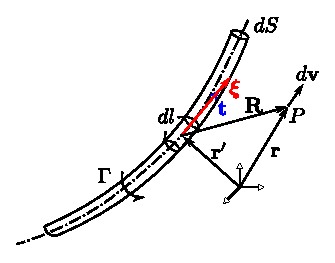
\includegraphics[scale=1.8]{figure/chapter4/4-1-4.eps}
%\caption{\label{fig:blue_rectangle} Rectangle}
\end{figure}
From Helmholtz Theorem
\[
\boldsymbol{\xi}\cdot\mathbf{t}dS = \Gamma = \text{ constant}
\]
From \eqref{eq: 4-5-5}
\begin{equation}
\Longrightarrow
d\mathbf{v}(\mathbf{r}) = \frac{1}{4\pi} \frac{\boldsymbol{\xi}(\mathbf{r'})d\volume_{r'}\times\mathbf{R}}{R^3} \vc{=}{\footnotemark}{} \frac{1}{4\pi}\frac{\Gamma dl\mathbf{t}\times \mathbf{R}}{R^3}
\label{eq: 4-5-6}
\end{equation}
Since $\Gamma$ is constant
\begin{equation}
\mathbf{v}(\mathbf{r}) = \frac{\Gamma}{4\pi}\int\frac{\mathbf{t}\times\mathbf{R}}{R^3}dl
\label{eq: 4-5-7}
\end{equation}
\footnotetext{$\boldsymbol{\xi}(\mathbf{r'})d\volume_{r'} = \boldsymbol{\xi}\left(\mathbf{t}dS\cdot d\mathbf{l}\right) = \boldsymbol{\xi}\left(\mathbf{t}dS\cdot\frac{\boldsymbol{\xi}}{\xi}dl\right) = \boldsymbol{\xi}\frac{\Gamma}{\xi}dl = \Gamma \mathbf{t}dl$}\\
\item Straight Infinite-long vortex filament

\tdplotsetmaincoords{60}{110}
\begin{center}

\begin{tikzpicture}[scale=3, tdplot_main_coords]
    \coordinate (O) at (0,0,0);
    \tdplotsetcoord{inf}{2}{0}{90} 
    \tdplotsetcoord{ninf}{-0.5}{0}{-90} 
    \tdplotsetcoord{P}{2}{30}{70}
    \tdplotsetcoord{l}{0.5}{0}{90} 
    \tdplotsetcoord{dl}{0.8}{0}{90} 
    \tdplotsetcoord{t}{1.1}{0}{90} 
    \draw plot [mark=*, mark size=0.5] (P) node [right] {$P$}; 
    \draw plot [mark=*, mark size=0.5] (l) ; 
    \draw plot [mark=*, mark size=0.5] (t) ; 
	\draw plot [mark=*, mark size=0.5] (O) node [left] {$O$}; 
    \draw[-{Latex[length=2mm]}] (O) -- (inf) node [at end, above]{$\infty$};
    \draw[-{Latex[length=2mm]}] (O) -- (ninf) node [at end, below]{$-\infty$};
    \draw[thick,-{Latex[length=2mm]}] (O) -- (P) node [pos=0.5, anchor=north]{$\mathbf{r}$} ;
    \draw[thick, -{Latex[length=2mm]}] (O) -- (l) node [pos=0.7, anchor=east]{$\mathbf{r'}$} node [pos=0.7, anchor=west]{$l$} ;
    \draw[ {Latex[length=2mm]}-{Latex[length=2mm]}] (l) -- (dl) node [pos=0.5, anchor=east]{$dl$} ;
    \draw[thick, -{Latex[length=2mm]}] (dl) -- (t) node [pos=0.7, anchor=east]{$\mathbf{t}$}  ;
    \draw[thick, -{Latex[length=2mm]}] (l) -- (P) node [pos=0.5, anchor=south]{$\mathbf{R}$} ;

    \draw[-] (P) -- (Pz) node [pos=0.5, anchor=south] {${r_0}$};

	\draw pic["$\alpha$", draw=red, text=red, <->, angle eccentricity=1.2, angle radius=1.6cm] {angle=P--O--l};
	\draw pic["$\theta$", draw=red, text=red, <->, angle eccentricity=1.2, angle radius=1cm] {angle=P--l--inf};
	\coordinate (e) at (-1.8794,0.684,0);
	\draw[thick, -{Latex[length=2mm]}] (P) -- (e) node [right, at end]{$\mathbf{e}$} ;
	\coordinate (v1) at ($(Pz) + (0,0,0.1)$);
	\coordinate (v3) at ($(Pz)!0.2!(P)$);
	\coordinate (v2) at (0.0684,0.18794,1.832);
	\draw [thick, red] (v1) -- (v2) -- (v3);
%	\draw [red] (Pz)  ++(0,0,0.1) -- ($(x)!0.25!(vtip)$)--(a);  
\end{tikzpicture}
\end{center}
\begin{equation}
\mathbf{t}\times\mathbf{R} = R\sin\theta\mathbf{e}
\label{eq: 4-5-8}
\end{equation}
where $\mathbf{e}$ is unit vector into board.\\
From \eqref{eq: 4-5-7}
\begin{align}
\mathbf{v}(\mathbf{r}) 
&= \frac{\Gamma}{4\pi}\int_{-\infty}^\infty\mathbf{e}\frac{\sin\theta}{R^2}dl
\tag{$\ast$}
\label{eq: 4-5-*} \\
&\vc{=}{\text{in this}}{\text{case}}\mathbf{e}\frac{\Gamma}{4\pi}\int_{-\infty}^{\infty}\frac{\sin\theta}{R^2}dl \vc{=}{\footnotemark}{} \mathbf{e}\frac{\Gamma}{4\pi}\int_0^\pi\frac{\sin\theta}{r_0}d\theta\nonumber  \\
&= \frac{\Gamma}{2\pi r_0}\mathbf{e}\label{eq: 4-5-88}
\end{align}
\footnotetext{From geometry, $\displaystyle\frac{r\cos\alpha - l}{r_0} = \cot\theta\Longrightarrow dl = \frac{r_0d\theta}{\sin^2\theta}$ and $\displaystyle R^2 = \frac{r_0^2}{\sin^2\theta}$}
\begin{note}\mbox{}\\
\begin{enumerate}[label = \protect\circled{\arabic*}]
\item For semi-infinite long vortex filament
%----------------------
\begin{minipage}{0.4\textwidth}
\begin{equation}
\mathbf{v}(\mathbf{r}) = \frac{\Gamma}{4\pi r_0}\left(1+\cos\theta_0\right)\mathbf{e}
\label{eq: 4-5-9}
\end{equation}
\[
\left(\int_{\theta = 0}^{\theta = \pi}\left(\cdots\right)d\theta\longrightarrow\int_{\theta = \theta_0}^{\theta = \pi}\left(\cdots\right)d\theta\right)
\]
\end{minipage} \hfill
\begin{minipage}{0.3\textwidth}
\tdplotsetmaincoords{90}{0}
\begin{center}
\begin{tikzpicture}[scale=2, tdplot_main_coords]
    \coordinate (O) at (0,0,0);
    \tdplotsetcoord{inf}{2}{0}{90} 
    \tdplotsetcoord{ninf}{-0.5}{0}{-90} 
    \tdplotsetcoord{P}{2}{30}{70}
    \tdplotsetcoord{l}{0.5}{0}{90} 
    \tdplotsetcoord{dl}{0.8}{0}{90} 
    \tdplotsetcoord{t}{1.1}{0}{90} 
    \draw plot [mark=*, mark size=0.5] (P) node [right] {$P$}; 
	\draw plot [mark=*, mark size=0.5] (O) node [left] {$O$}; 
    \draw[-{Latex[length=2mm]}] (O) -- (inf) node [at end, above]{$\infty$};
    \draw[thick,-{Latex[length=2mm]}] (O) -- (P) node [pos=0.5, anchor=west]{$\mathbf{r}$} ;


    \draw[-] (P) -- (Pz) node [pos=0.5, anchor=south] {${r_0}$};
	\coordinate (v1) at ($(Pz) + (0,0,0.1)$);
	\coordinate (v3) at ($(Pz)!0.2!(P)$);
	\coordinate (v2) at (0.0684,0.18794,1.832);
	\draw [thick, red] (v1) -- (v2) -- (v3);
	\draw pic["$\theta_0$", draw=red, text=red, <->, angle eccentricity=1.6, angle radius=1.6cm] {angle=P--O--Pz};
\end{tikzpicture}
\end{center}
\end{minipage}\\
%----------------------
\item For a segment of vortex filament
%----------------------
\begin{minipage}{0.4\textwidth}
\begin{equation}
\begin{aligned}
\mathbf{v}(\mathbf{r})
&= \frac{\Gamma}{4\pi r_0}\left(\cos\theta_1-\cos\theta_2\right) \\
&= \frac{\Gamma}{4\pi r_0}\left(\cos\theta_1+\cos\theta_3\right)
\end{aligned}
\label{eq: 4-5-9}
\end{equation}
\end{minipage} \hfill
\begin{minipage}{0.3\textwidth}
\tdplotsetmaincoords{90}{0}
\begin{center}
\begin{tikzpicture}[scale=2, tdplot_main_coords]
    \coordinate (O) at (0,0,0);
    \tdplotsetcoord{inf}{2.3}{0}{90} 
    \tdplotsetcoord{ninf}{-0.5}{0}{-90} 
    \tdplotsetcoord{P}{2}{60}{50}
    \tdplotsetcoord{l}{0.5}{0}{90} 
    \tdplotsetcoord{dl}{0.8}{0}{90} 
    \tdplotsetcoord{t}{1.1}{0}{90} 
    \tdplotsetcoord{tt}{1.7}{0}{90} 
    \draw plot [mark=*, mark size=0.5] (P) node [right] {$P$}; 
    \draw plot [mark=*, mark size=0.5] (tt) ; 
	\draw plot [mark=*, mark size=0.5] (O) node [left] {$O$}; 
    \draw[dashed] (tt) -- (inf);
    \draw[-] (O) -- (tt);
    \draw[thick,-{Latex[length=2mm]}] (O) -- (P) node [pos=0.5, anchor=west]{$\mathbf{r}$} ;
	\draw[thick,-{Latex[length=2mm]}] (tt) -- (P) ;

    \draw[-] (P) -- (Pz) node [pos=0.5, anchor=south] {${r_0}$};
	\coordinate (v1) at ($(Pz) + (0,0,0.1)$);
	\coordinate (v3) at ($(Pz)!0.2!(P)$);
	\coordinate (v2) at (0.22266,0.26536,1.1);
	\draw [thick, red] (v1) -- (v2) -- (v3);
	\draw pic["$\theta_1$", draw=red, text=red, <->, angle eccentricity=1.3, angle radius=1.2cm] {angle=P--O--Pz};
	\draw pic["$\theta_3$", draw=red, text=red, <->, angle eccentricity=1.4, angle radius=0.7cm] {angle=O--tt--P};
	\draw pic["$\theta_2$", draw=red, text=red, <->, angle eccentricity=1.3, angle radius=1.2cm] {angle=P--tt--inf};
\end{tikzpicture}
\end{center}
\end{minipage}\\
%----------------------
\end{enumerate}
\end{note}
\item (Concentrated) Horseshoe Vortex filament
\begin{figure}[H]
\centering
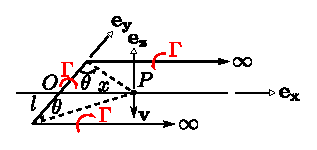
\includegraphics[scale=1.8]{figure/chapter4/4-1-5.eps}
%\caption{\label{fig:blue_rectangle} Rectangle}
\end{figure}
\[
\mathbf{v} = -\mathbf{e_z}\left[\frac{\Gamma}{4\pi x}\left(\cos\theta + \cos\theta\right) + 2\frac{\Gamma}{4\pi l}\left(1+\sin\theta\right)\right]
\]
or
\begin{equation}
\mathbf{v}(x) = -\mathbf{e_z}\frac{\Gamma}{2\pi l}\left[1 + \frac{\sqrt{l^2+x^2}}{x}\right]
\label{eq: 4-5-11}
\end{equation}
\begin{itemize}
\item In thin airfoil theory
\begin{figure}[H]
\centering
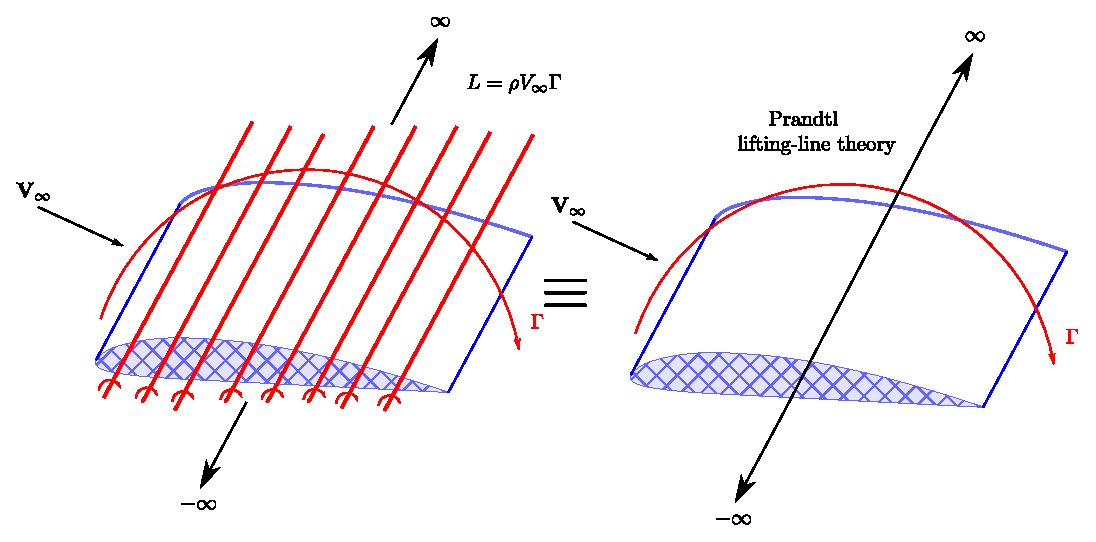
\includegraphics[scale=1.0]{figure/chapter4/4-1-6.eps}
%\caption{\label{fig:blue_rectangle} Rectangle}
\end{figure}
\item In 3D (finite wing)
\begin{figure}[H]
\centering
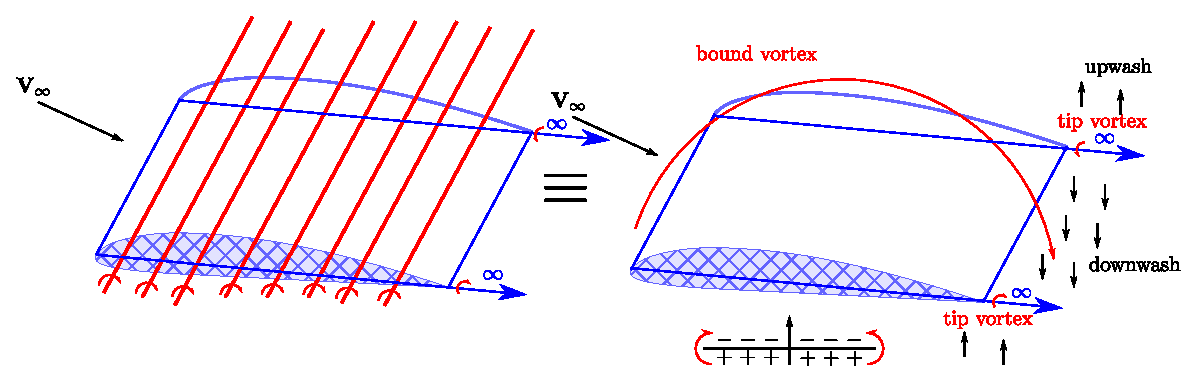
\includegraphics[scale=0.9]{figure/chapter4/4-1-7.eps}
%\caption{\label{fig:blue_rectangle} Rectangle}
\end{figure}
\item In real viscous flow
\begin{figure}[H]
\centering
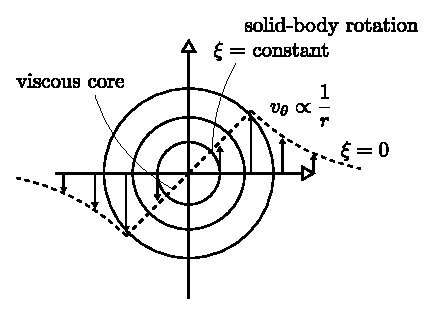
\includegraphics[scale=0.9]{figure/chapter4/4-1-8.eps}
%\caption{\label{fig:blue_rectangle} Rectangle}
\end{figure}
which is Rankine vortex (or Circular vortex). 
\end{itemize}
\end{itemize}
\subsubsection{Velocity Induced by Concentrated Vorticity- Concentrated Vortex Sheet}
%----------------------
\begin{minipage}{0.4\textwidth}
\begin{figure}[H]
\centering
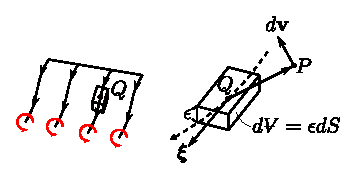
\includegraphics[scale=1.3]{figure/chapter4/4-1-9.eps}
%\caption{\label{fig:blue_rectangle} Rectangle}
\end{figure}
\end{minipage} \hfill
\begin{minipage}{0.5\textwidth}
\[
\boldsymbol{\xi}d\volume = \boldsymbol{\xi}\epsilon dS
\]
as $\epsilon\to 0$, let $\abs{\boldsymbol{\xi}}\to\infty$\\
so that $\abs{\boldsymbol{\xi}\epsilon} = \abs{\boldsymbol{\gamma}}=$ constant at point $Q$
\end{minipage}\\
%----------------------
Biot-Savart law:
\begin{equation}
d\mathbf{v}(\mathbf{r}) = \frac{1}{4\pi}\frac{\boldsymbol{\gamma}(\mathbf{r}')dS\times\mathbf{R}}{R^3}
\label{eq: 4-5-11}
\end{equation}
What is $\abs{\boldsymbol{\gamma}}$?
\begin{figure}[H]
\centering
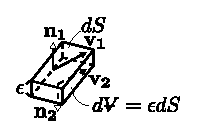
\includegraphics[scale=1.8]{figure/chapter4/4-1-10.eps}
%\caption{\label{fig:blue_rectangle} Rectangle}
\end{figure}
Now
\[
\boldsymbol{\xi}d\volume = \nabla\times\mathbf{v}d\volume\vc{=}{\footnotemark}{}\oiint_{\Delta S}\mathbf{n}\times \mathbf{v}dS
\]
\footnotetext{integral definition of $\nabla\times\mathbf{v}$}
Hence
\begin{align*}
\boldsymbol{\xi}d\volume
&= \lim_{\epsilon\to 0}\boldsymbol{\xi}\epsilon dS\\
&= \lim_{\epsilon\to 0}\oiint_{\Delta S}\mathbf{n}\times\mathbf{v}dS \\
&= \left(\mathbf{n_1}\times\mathbf{v}_1 + \mathbf{n_2}\times\mathbf{v}_2\right)dS
\end{align*}
\[
\Longrightarrow\boldsymbol{\gamma} = \mathbf{n}\times\left(\mathbf{v_1}-\mathbf{v_2}\right)
\]
but $\left(\mathbf{v_1}-\mathbf{v_2}\right)\perp\mathbf{n}$\\
hence
\begin{equation}
\abs{\boldsymbol{\gamma}} = \abs{\mathbf{v_1}-\mathbf{v_2}} = \abs{u_1-u_2}
\label{eq: 4-5-12}
\end{equation}\\
\vspace{5em}
%----------------------
\begin{minipage}{0.4\textwidth}
\begin{tikzpicture}
\begin{scope}[scale=2,transform canvas]
\coordinate (O) at (0,0);
\draw[-] (O) -- (3,0);

\foreach \v in {0,0.4,0.8,1.2,1.6,2.0,2.4,2.8}{
    \fill[color=red] ($(\v, 0)$) circle[radius=1pt] ;
    \draw [color=red,-{Latex[length=1mm]}, rotate=0] (\v,-0.2) arc [start angle=270, end angle=450, x radius=0.2cm, y radius=0.2cm] ; 
}
\node [red, below] at (0.2,-0.2) {$dx$};
\coordinate (VO) at (1.2,0);
\coordinate (VOtop) at (1.2,1.5);
\coordinate (VObuttom) at (1.2,-1.5);
\draw[-] ($(VO) + (0,-1.5)$) -- ($(VO) + (0,1.5)$);
\foreach \v in {0.2,0.4,0.6,0.8}{
       \draw[->]  ($(VO)!\v!(VOtop)$) -- ($(VO)!\v!(VOtop) + (1,0)$);    
}
\draw[-] ($(VO) + (1,0)$) -- ($(VO) + (1,1.5)$) node [above left]{$u_1$};
\foreach \v in {0.2,0.4,0.6,0.8}{
       \draw[->]  ($(VO)!\v!(VObuttom)$) -- ($(VO)!\v!(VObuttom) + (1.5,0)$);    
}
\draw[-] ($(VO) + (1.5,0)$) -- ($(VO) + (1.5,-1.5)$) node [below left]{$u_2$};
\end{scope}
\end{tikzpicture}
\end{minipage} \hfill
\begin{minipage}{0.5\textwidth}
\[
d\Gamma = \left(u_2-u_1\right)dx = \gamma dx
\]
\end{minipage}\\
%----------------------
\vspace{8em}
\begin{itemize}
\item Vortex Sheet of Straight, Infinite-long Vortex Filament\\
\vspace{8em}
%----------------------
\begin{minipage}{0.4\textwidth}
\begin{tikzpicture}[scale=2,transform canvas]
\begin{scope}[scale=2,transform canvas]
    \filldraw[color=blue!60, fill=blue!10, line width=0.04mm] 
(1.0000000,0.0005993) -- 
(0.9900000,0.0029690) --
(0.9800000,0.0053335) -- 
(0.9700000,0.0076868) -- 
(0.9600000,0.0100232) -- 
(0.9400000,0.0146239) -- 
(0.9200000,0.0191156) -- 
(0.9000000,0.0235025) -- 
(0.8800000,0.0277891) -- 
(0.8600000,0.0319740) -- 
(0.8400000,0.0360536) -- 
(0.8200000,0.0400245) -- 
(0.8000000,0.0438836) -- 
(0.7800000,0.0476281) -- 
(0.7600000,0.0512565) -- 
(0.7400000,0.0547675) -- 
(0.7200000,0.0581599) -- 
(0.7000000,0.0614329) -- 
(0.6800000,0.0645843) -- 
(0.6600000,0.0676046) -- 
(0.6400000,0.0704822) -- 
(0.6200000,0.0732055) -- 
(0.6000000,0.0757633) -- 
(0.5800000,0.0781451) -- 
(0.5600000,0.0803480) -- 
(0.5400000,0.0823712) -- 
(0.5200000,0.0842145) -- 
(0.5000000,0.0858772) -- 
(0.4800000,0.0873572) -- 
(0.4600000,0.0886427) -- 
(0.4400000,0.0897175) -- 
(0.4200000,0.0905657) -- 
(0.4000000,0.0911712) -- 
(0.3800000,0.0915212) -- 
(0.3600000,0.0916266) -- 
(0.3400000,0.0915079) -- 
(0.3200000,0.0911857) -- 
(0.3000000,0.0906804) -- 
(0.2800000,0.0900016) -- 
(0.2600000,0.0890840) -- 
(0.2400000,0.0878308) -- 
(0.2200000,0.0861433) -- 
(0.2000000,0.0839202) -- 
(0.1800000,0.0810687) -- 
(0.1600000,0.0775707) -- 
(0.1400000,0.0734360) -- 
(0.1200000,0.0686204) -- 
(0.1000000,0.0629981) -- 
(0.0800000,0.0564308) -- 
(0.0600000,0.0487571) -- 
(0.0500000,0.0442753) -- 
(0.0400000,0.0391283) -- 
(0.0300000,0.0330215) -- 
(0.0200000,0.0253735) -- 
(0.0120000,0.0178581) -- 
(0.0080000,0.0137350) -- 
(0.0040000,0.0089238) -- 
(0.0020000,0.0058025) -- 
(0.0010000,0.0037271) -- 
(0.0005000,0.0023390) -- 
(0.0000000,0.0000000) coordinate (y) -- 
(0.0005000,-.0046700) -- 
(0.0010000,-.0059418) -- 
(0.0020000,-.0078113) -- 
(0.0040000,-.0105126) -- 
(0.0080000,-.0142862) -- 
(0.0120000,-.0169733) -- 
(0.0200000,-.0202723) -- 
(0.0300000,-.0226056) -- 
(0.0400000,-.0245211) -- 
(0.0500000,-.0260452) -- 
(0.0600000,-.0271277) -- 
(0.0800000,-.0284595) -- 
(0.1000000,-.0293786) -- 
(0.1200000,-.0299633) -- 
(0.1400000,-.0302404) -- 
(0.1600000,-.0302546) -- 
(0.1800000,-.0300490) -- 
(0.2000000,-.0296656) -- 
(0.2200000,-.0291445) -- 
(0.2400000,-.0285181) -- 
(0.2600000,-.0278164) -- 
(0.2800000,-.0270696) -- 
(0.3000000,-.0263079) -- 
(0.3200000,-.0255565) -- 
(0.3400000,-.0248176) -- 
(0.3600000,-.0240870) -- 
(0.3800000,-.0233606) -- 
(0.4000000,-.0226341) -- 
(0.4200000,-.0219042) -- 
(0.4400000,-.0211708) -- 
(0.4600000,-.0204353) -- 
(0.4800000,-.0196986) -- 
(0.5000000,-.0189619) -- 
(0.5200000,-.0182262) -- 
(0.5400000,-.0174914) -- 
(0.5600000,-.0167572) -- 
(0.5800000,-.0160232) -- 
(0.6000000,-.0152893) -- 
(0.6200000,-.0145551) -- 
(0.6400000,-.0138207) -- 
(0.6600000,-.0130862) -- 
(0.6800000,-.0123515) -- 
(0.7000000,-.0116169) -- 
(0.7200000,-.0108823) -- 
(0.7400000,-.0101478) -- 
(0.7600000,-.0094133) -- 
(0.7800000,-.0086788) -- 
(0.8000000,-.0079443) -- 
(0.8200000,-.0072098) -- 
(0.8400000,-.0064753) -- 
(0.8600000,-.0057408) -- 
(0.8800000,-.0050063) -- 
(0.9000000,-.0042718) -- 
(0.9200000,-.0035373) -- 
(0.9400000,-.0028028) -- 
(0.9600000,-.0020683) -- 
(0.9700000,-.0017011) -- 
(0.9800000,-.0013339) -- 
(0.9900000,-.0009666) -- 
(1.0000000,-.0005993) coordinate (x);
%
\draw[color=blue!60 ,pattern=hatch, pattern color=blue!60, hatch size=10pt, hatch angle=0]
(1.0000000,0.0005993) -- 
(0.9900000,0.0029690) -- 
(0.9800000,0.0053335) -- 
(0.9700000,0.0076868) -- 
(0.9600000,0.0100232) -- 
(0.9400000,0.0146239) -- 
(0.9200000,0.0191156) -- 
(0.9000000,0.0235025) -- 
(0.8800000,0.0277891) -- 
(0.8600000,0.0319740) -- 
(0.8400000,0.0360536) -- 
(0.8200000,0.0400245) -- 
(0.8000000,0.0438836) -- 
(0.7800000,0.0476281) -- 
(0.7600000,0.0512565) -- 
(0.7400000,0.0547675) -- 
(0.7200000,0.0581599) -- 
(0.7000000,0.0614329) -- 
(0.6800000,0.0645843) -- 
(0.6600000,0.0676046) -- 
(0.6400000,0.0704822) -- 
(0.6200000,0.0732055) -- 
(0.6000000,0.0757633) -- 
(0.5800000,0.0781451) -- 
(0.5600000,0.0803480) -- 
(0.5400000,0.0823712) -- 
(0.5200000,0.0842145) -- 
(0.5000000,0.0858772) -- 
(0.4800000,0.0873572) -- 
(0.4600000,0.0886427) -- 
(0.4400000,0.0897175) -- 
(0.4200000,0.0905657) -- 
(0.4000000,0.0911712) -- 
(0.3800000,0.0915212) -- 
(0.3600000,0.0916266) -- 
(0.3400000,0.0915079) -- 
(0.3200000,0.0911857) -- 
(0.3000000,0.0906804) -- 
(0.2800000,0.0900016) -- 
(0.2600000,0.0890840) -- 
(0.2400000,0.0878308) -- 
(0.2200000,0.0861433) -- 
(0.2000000,0.0839202) -- 
(0.1800000,0.0810687) -- 
(0.1600000,0.0775707) -- 
(0.1400000,0.0734360) -- 
(0.1200000,0.0686204) -- 
(0.1000000,0.0629981) -- 
(0.0800000,0.0564308) -- 
(0.0600000,0.0487571) -- 
(0.0500000,0.0442753) -- 
(0.0400000,0.0391283) -- 
(0.0300000,0.0330215) -- 
(0.0200000,0.0253735) -- 
(0.0120000,0.0178581) -- 
(0.0080000,0.0137350) -- 
(0.0040000,0.0089238) -- 
(0.0020000,0.0058025) -- 
(0.0010000,0.0037271) -- 
(0.0005000,0.0023390) -- 
(0.0000000,0.0000000) -- 
(0.0005000,-.0046700) -- 
(0.0010000,-.0059418) -- 
(0.0020000,-.0078113) -- 
(0.0040000,-.0105126) -- 
(0.0080000,-.0142862) -- 
(0.0120000,-.0169733) -- 
(0.0200000,-.0202723) -- 
(0.0300000,-.0226056) -- 
(0.0400000,-.0245211) -- 
(0.0500000,-.0260452) -- 
(0.0600000,-.0271277) -- 
(0.0800000,-.0284595) -- 
(0.1000000,-.0293786) -- 
(0.1200000,-.0299633) -- 
(0.1400000,-.0302404) -- 
(0.1600000,-.0302546) -- 
(0.1800000,-.0300490) -- 
(0.2000000,-.0296656) -- 
(0.2200000,-.0291445) -- 
(0.2400000,-.0285181) -- 
(0.2600000,-.0278164) -- 
(0.2800000,-.0270696) -- 
(0.3000000,-.0263079) -- 
(0.3200000,-.0255565) -- 
(0.3400000,-.0248176) -- 
(0.3600000,-.0240870) -- 
(0.3800000,-.0233606) -- 
(0.4000000,-.0226341) -- 
(0.4200000,-.0219042) -- 
(0.4400000,-.0211708) -- 
(0.4600000,-.0204353) -- 
(0.4800000,-.0196986) -- 
(0.5000000,-.0189619) -- 
(0.5200000,-.0182262) -- 
(0.5400000,-.0174914) -- 
(0.5600000,-.0167572) -- 
(0.5800000,-.0160232) -- 
(0.6000000,-.0152893) -- 
(0.6200000,-.0145551) -- 
(0.6400000,-.0138207) -- 
(0.6600000,-.0130862) -- 
(0.6800000,-.0123515) -- 
(0.7000000,-.0116169) -- 
(0.7200000,-.0108823) -- 
(0.7400000,-.0101478) -- 
(0.7600000,-.0094133) -- 
(0.7800000,-.0086788) -- 
(0.8000000,-.0079443) -- 
(0.8200000,-.0072098) -- 
(0.8400000,-.0064753) -- 
(0.8600000,-.0057408) -- 
(0.8800000,-.0050063) -- 
(0.9000000,-.0042718) -- 
(0.9200000,-.0035373) -- 
(0.9400000,-.0028028) -- 
(0.9600000,-.0020683) -- 
(0.9700000,-.0017011) -- 
(0.9800000,-.0013339) -- 
(0.9900000,-.0009666) -- 
(1.0000000,-.0005993);
\end{scope}
\coordinate (z) at (y |- x);
\draw [color=red,-{Latex[length=2mm]}, rotate=0] (-0.2,-0.3) arc [start angle=180, end angle=0, x radius=1.2cm, y radius=1cm] node[right]{$\Gamma$}; 
\draw[-{Latex[length=2mm]}] (1,0) -- (1,1) node[above]{$L$};
\end{tikzpicture}
\end{minipage} \hfill
\begin{minipage}{0.4\textwidth}
\begin{tikzpicture}[scale=2,transform canvas]
\foreach \v/\l/\w in {0/A/a,0.4/B/b,0.8/C/c,1.2/D/d,1.6/E/e,2.0/F/f,2.4/G/g,2.8/H/h}{
    \fill[color=red] ($(\v, 0)$) circle[radius=1pt] ;
    \draw [color=red,-{Latex[length=1mm]}, rotate=0] (\v,0.2) arc [start angle=90, end angle=-90, x radius=0.2cm, y radius=0.2cm] ;
    \coordinate (\w) at (\v, 0);
    \coordinate (\l) at ($(0.5+\v, 1)$);
    \draw[<->] (\l) -- ($(\l)!2.5cm!(\w)$) ;
}
% \node (a) {$a$};
% \node (A) {$A$};
\node [below] at (1.2,-1.2) {$-\infty$};
\node [above] at (1.5,1.2) {$\infty$};
\end{tikzpicture}
\end{minipage}\\
%----------------------
\vspace{8em}
\begin{tikzpicture}[scale=2,transform canvas]
\foreach \v in {0,0.4,0.8,1.2,1.6,2.0,2.4,2.8}{
    \fill[color=red] ($(\v, 0)$) circle[radius=1pt] ;
    \draw [color=red,-{Latex[length=1mm]}, rotate=0] (\v,0.2) arc [start angle=90, end angle=-90, x radius=0.2cm, y radius=0.2cm] ;
    \draw[-,color=red] (-0.4,0) -- (3.4,0);
}
\draw[-{Latex[length=2mm]}] (0.8,0.3) -- ($(0.8,0.3)+(1,0)$) node [above] {$u_1$};
\draw[-{Latex[length=2mm]}] (0.8,-0.3) -- ($(0.8,-0.3)+(0.5,0)$) node [below] {$u_2$};
\draw[thick,-,color=blue] (0.8,0.3) -- (0.8,-0.3) node [left] {$\epsilon$};
% \node (a) {$\epsilon$};
% \node (A) {$A$};
\draw [arrows = {-Latex[color=black, fill=white, length=3mm]}] (5,0) -- (6,0) node [at end, right] {$x$};
\draw [arrows = {-Latex[color=black, fill=white, length=3mm]}] (5,0) -- (5,1) node [at end, left] {$y$};
\end{tikzpicture}
\vspace{3em}
\[
d\Gamma = \left(u_1-u_2\right)dx = \gamma dx
\]
in general
\begin{equation}
\gamma(x) = u_1(x) - u_2(x)
\label{eq: 4-5-13}
\end{equation}
%----------------------
\begin{minipage}{0.4\textwidth}
\begin{tikzpicture}
\draw [arrows = {-Latex[color=black, fill=white, length=3mm]}] (0,0,0) -- (1,0,0) node [at end, above left] {$x$};
\draw [arrows = {-Latex[color=black, fill=white, length=3mm]}] (0,0,0) -- (0,1,0) node [at end, left] {$y$};
\draw [arrows = {-Latex[color=black, fill=white, length=3mm]}] (0,0,0) -- (0,0,1) node [at end, left] {$z$};
\fill[color=black] ($(1.5, 0)$) circle[radius=1pt] ;
\draw [color=red,-{Latex[length=1mm]}, rotate=0] (1.5,0.2) arc [start angle=90, end angle=-90, x radius=0.2cm, y radius=0.2cm] ;
\draw[-{Latex[length=2mm]}] (0,0) -- ($(0,0)+(1.5,0)$) node [below] {${r'} = x'$};
\draw[-] (0,0) -- (3,0) ;
\node [red, below] at (1.5,-0.5) {$dx$};
\node [red, below] at (1.5,-1) {$d\Gamma = \gamma(x')dx'$};
\coordinate (P) at (2,1);
\fill[color=black] (P) circle[radius=1pt] ;
\draw[-{Latex[length=2mm]}, rotate=0]{} (0,0,0) -- (P) node[pos=0.5, anchor=south]{$\mathbf{r}$} node[at end, above]{$P(x,y)$};
\draw[-{Latex[length=2mm]}, rotate=0]{} (1.5,0) -- (P) node[pos=0.5, anchor=west]{$\mathbf{R}$} ;
\draw[color=blue,-{Latex[length=2mm]}, rotate=0]{} (P) -- (4,-2) node[at end, right]{$d\mathbf{v}$} ;
\end{tikzpicture}
\end{minipage} \hfill
\begin{minipage}{0.4\textwidth}
Recall, from \eqref{eq: 4-5-88}\\
$\displaystyle\mathbf{v}(\mathbf{r}) = \frac{\Gamma}{2\pi R}\mathbf{e}$ for a single concentrated vortex filament
\[
\Longrightarrow d\mathbf{v} = \frac{d\Gamma}{2\pi R}\mathbf{e} = \frac{\gamma(x')dx'}{2\pi R}\mathbf{e}
\]
\end{minipage}\\
%----------------------
\vspace{2em}
\begin{equation}
\mathbf{v}(x,y) = \frac{1}{2\pi}\int\left[\frac{\gamma(x')dx'}{R(x')}\mathbf{e}\right]
\label{eq: 4-5-13}
\end{equation}
\begin{exercise}\mbox{}\\
Show that if $\gamma(x)\equiv\gamma = $ constant along $-\infty<x<\infty$, then
\begin{align*}
\mathbf{v}(x,y)
&= \frac{\gamma}{2}\mathbf{e_x}\text{ at $+$ side} \\
&= -\frac{\gamma}{2}\mathbf{e_x}\text{ at $-$ side} \\
\end{align*}

\begin{center}
\begin{tikzpicture}[scale=1,transform canvas]
\node[below left] at (0,0) {$O$};
\fill[color=black] ($(1.5, 0)$) circle[radius=1pt] ;
\draw [color=red,-{Latex[length=1mm]}, rotate=0] (1.5,0.2) arc [start angle=90, end angle=-90, x radius=0.2cm, y radius=0.2cm] ;
\draw[-{Latex[length=2mm]}] (0,0) -- ($(0,0)+(1.5,0)$) node [below] {${r'} = x'$};
\draw[-] (0,0) -- (3,0) ;
\node [red, below] at (1.5,-0.5) {$dx'$};
\coordinate (P) at (2,1);
\coordinate (OO) at (1.5,0);
\coordinate (end) at (3,0);
\coordinate (R) at ($(1.5,0)+(-1,0.5)$);
\fill[color=black] (P) circle[radius=1pt] ;
\fill[color=black] (O) circle[radius=1pt] ;
\draw[-{Latex[length=2mm]}, rotate=0]{} (1.5,0) -- (P) node[pos=0.7, anchor=east]{$\mathbf{R}$} node[at end, above]{$P(x,y)$} ;
\draw[-{Latex[length=2mm]}, rotate=0]{} (1.5,0) -- ($(1.5,0)+(-1,0.5)$) node[pos=1.0, anchor=east]{$\mathbf{e}$} ;
\coordinate (e) at ($(1.5,0)+(-1,0.5)$);
\draw pic["$\theta$", draw=red, text=red, <->, angle eccentricity=1.4, angle radius=0.7cm] {angle=end--OO--P};
\coordinate (A) at ($(OO)!0.2!(P)$);
\coordinate (B) at ($(OO)!0.2!(R)$);
\draw (A) -- ($(A)+(-0.2,0.1)$) -- (B);
\end{tikzpicture}
\end{center}
\vspace{3em}
\begin{align*}
u &= \frac{\gamma}{2}\int_{-\infty}^{\infty}\frac{-\cos(\pi/2-\theta)}{\sqrt{\left(x-x'\right)^2+y^2}}dx' 
= \frac{\gamma}{2\pi}\underbrace{\frac{y}{\left(x-x'\right)^2+y^2}dx'}_{=\pi} \\
&=\frac{\gamma}{2}
\end{align*}

\end{exercise}

\end{itemize}